%&latexf
\documentclass[a4paper]{article}
\usepackage{color}
\setlength{\hoffset}{-0.5in}\hoffset-0.5in
\setlength{\textwidth}{15cm}
\usepackage{hyperref}
\usepackage{amsmath, amsfonts, amsthm, amssymb}
\usepackage{verbatim}
\usepackage{stmaryrd}
\usepackage{fancyhdr}
\usepackage{color}
%\usepackage[dvips]{graphicx}
\usepackage{subfigure}
%%%%%%%%%%%%%%%%%%%%%%%%%%%%%%%%%%%
\usepackage{dsfont}
\usepackage{enumerate}
\usepackage{multirow}
\usepackage{float}
\usepackage{graphicx}
\usepackage{listings}

%%%%%%%%%%%%%%%%%%%%%%%%%%%%%%%%%%%
\linespread{1.5}
%\font\twelvemsb=msbm10 at 12pt
\newfam\msbfam
%\textfont\msbfam=\twelvemsb
\def\Bbb#1{\fam\msbfam\relax#1}

\topmargin = 20pt
\voffset = -20pt
\addtolength{\textheight}{2cm}
\newtheorem{theorem}{Theorem}[section]
\newtheorem{exa}{Example}[section]
\newtheorem{corollary}[theorem]{Corollary}
\newtheorem{lemma}[theorem]{Lemma}
\newtheorem{proposition}[theorem]{Proposition}

\theoremstyle{definition}
\newtheorem{definition}[theorem]{Definition}
\newtheorem{remark}[theorem]{Remark}
\newtheorem{notation}[theorem]{Notation}
\newtheorem{assumption}[theorem]{Assumption}
\newtheorem{conjecture}[theorem]{Conjecture}
%%%%%%%%%%%%%%%%%%%%%%%%%%%%%%%%%%%%%%%%%%%%%%%%%%%%%%%%%%%%%%
\newtheorem{condition}[theorem]{Condition}

\newcommand{\ind}{1\hspace{-2.1mm}{1}} %Indicator Function
\newcommand{\I}{\mathtt{i}}
\newcommand{\D}{\mathrm{d}}
\newcommand{\E}{\mathrm{e}}
\newcommand{\RR}{\mathbb{R}}
\newcommand{\sgn}{\mathrm{sgn}}
\newcommand{\atanh}{\mathrm{arctanh}}
\def\equalDistrib{\,{\buildrel \Delta \over =}\,}
\numberwithin{equation}{section}
\def\blue#1{\textcolor{blue}{#1}}
\def\red#1{\textcolor{red}{#1}}


\begin{document}
%The following commands include several pages which contain the front page, acknowledgements,...
\thispagestyle{empty}
\null\vskip0.2in%
\begin{center}
\LARGE{{\bf 
Optimal Portfolio Problems}}
\end{center}

\vspace{0.5cm}

\begin{center}
{\Large {\bf by}}\\
\mbox{} \\
{\Large {\bf Yueying Zhou (CID: 01230489)}}
\end{center}

\vspace{1cm}

\begin{center}
\large{\bf{Department of Mathematics \\ Imperial College London \\
London SW7 2AZ \\ United Kingdom}}
\end{center}



\vspace{9.5cm}

\begin{center}
\large{\bf{Thesis submitted as part of the requirements for the award of the \\
MSc in Mathematics and Finance, Imperial College London, 2016-2017}}
\end{center}

\vspace{2cm}


%\thispagestyle{empty}


\mbox{}\newline\vspace{10mm} \mbox{}\LARGE
%
{\bf Declaration} \normalsize \vspace{5mm}

The work contained in this thesis is my own work unless otherwise stated.

\bigskip
\bigskip
\bigskip


Signature and date: 


\newpage

\mbox{}\newline\vspace{10mm} \mbox{}\LARGE
%
{\bf Acknowledgements} \normalsize \vspace{5mm}

Firstly, I am deeply grateful to Dr. Pietro Siorpaes who is both my tutor in this academic year and my supervisor of this project. He gave me much ongoing guidance and support in this year. In particular, I am very appreciate his patience and constructive suggestions throughout this project, which make my thesis much better. The help from my supervisor is so huge and invaluable for me.

%Secondly, I am greatly thankful to Professor Nicholas Bingham who is a native speaker. He is so helpful and patient that gave me much help in English writing.

Additionally, I would also express my gratitude to Dr. Antoine Jacquier for his help on programming. When I met difficulties on coding, he helped me to find mistakes.

At last, I would like to thank my friend, Shuang Yang, and my parents, all of whom gave me great irreplaceable, ongoing encouragement and support while I did this project.







\mbox{}\newline\vspace{10mm} \mbox{}\LARGE
%
{\bf Abstract} \normalsize \vspace{5mm}

This paper aims to solve two kinds of optimal portfolio problems, the terminal wealth problem and the infinite-horizon consumption problem. Methods applied in this paper are the martingale method and the dynamic programming method. Additionally, we apply the finite difference method to all continuous-time problems in this paper so that we can conclude that this numerical method is feasible by comparing the estimated solutions with the closed forms from the dynamic programming method.

For the terminal wealth problem, we use the martingale method in discrete time, while using the dynamic programming method in both discrete and continuous times.

For the consumption problem, we discuss a basic problem, Merton's problem, and a variation of it, the problem with the habit formation model and preference for wealth. We apply only the dynamic programming method to both consumption problems. Furthermore, with the solution to these two problems, we can see the differences of the optimal expected utility of consumption with and without considering the exponentially-weighted historical
average of past consumption.






\newpage
%%%
\setcounter{tocdepth}{4}
%%%

\tableofcontents %% This includes the table of contents, which is organised automatically, 
 %% and used your section / subsection.
 
\newpage %%This simply means that the next part of text will start on a new page.

%%%%%%%%%%%%%%%%%%%%%%%%%%%%%%%%%%%%%%%%%%%%%%%%%%%%
\fancyhead{}
\fancyfoot{}
\pagestyle{fancy} 
\fancyhead[RO,LE]{\sffamily\small \thepage}
\fancyhead[LO,RE]{\sffamily\small \nouppercase{\rightmark}}
\renewcommand{\headrulewidth}{0.4pt}
\renewcommand{\footrulewidth}{0.0pt}
%%%%%%%%%%%%%%%%%%%%%%%%%%%%%%%%%%%%%%%%%%%%%%%%%%%%





%%%%%%%%%%%%%%%%%%%%%%%%%%%%%%%%%%%%%%%%%%%%%%%%%%%%
%%%%%%%%%%%%%%%%%%%%%%%%%%%%%%%%%%%%%%%%%%%%%%%%%%%%

\section{Introduction}
The research of portfolio selection problems starts from Markowitz (1952)~\cite{mark 52} who used the mean-variance method to solve the problems over one period. The objective in his paper is maximization of the expected return given a level of risk, i.e., variance. With this paper, he was awarded a Nobel Prize in economics.

During that period, Bellman (1954)~\cite{bellman 54} introduced the Bellman equation, which is the foundation of the dynamic programming method. Then Mossin (1968)~\cite{mossin 68} and Samuelson (1969)~\cite{sam 69} developed the dynamic programming method in discrete time. The key to this method is breaking a complex problem into simpler sub-problems. Its application to optimal investment is dividing time $T$ into a number of parts and solving the sub-problem at each short period.

At the same time, the dynamic programming method applied in continuous-time optimization problems is developed. Merton is a person whose work is regarded as the beginning point of continuous-time portfolio theory. His paper(1971)~\cite{merton} applied the stochastic control theory to the portfolio optimization problem by Hamilton-Jacobi-Bellman Equation of dynamic programming method, and gave explicit solutions for the consumption problem in infinite time. His approach is widely used in finance and is introduced in this paper.

After that, Harrison and Kreps (1979)~\cite{HK 79} introduced a different method to solve optimal portfolio problems, the martingale method. In that paper, they not only gave an example for the application to this method in discrete time but also discussed its application to the continuous-time problem. The key to this method is the stochastic calculus and convex optimization instead of the stochastic control theory which is applied in dynamic programming method. Karatzas et al. (2002)~\cite{completing} said that the idea of 'completing' the market begins with Karatzas et al. (1991)~\cite{KL 91}, in which they extended the martingale method to the incomplete market.

Another numerical method applied in this paper is the finite difference method which depends on the Taylor expansion, introduced by Taylor in 1715. This method has been applied for more than 200 years to approximate the solution to differential equations in many fields, such as physical sciences and engineering.

Later, these methods are applied to the more realistic models. In this paper, we would discuss about the optimal portfolio problem with habit formation model and preference for wealth, which origins from Xiao and Xu (2003)~\cite{c-i with wealth}. For the part of habit formation model, Constantinides (1990)~\cite{constantinides} discuss the consumption problem with habit formation model in a partial equilibrium model, while Sundaresan (1989)~\cite{Sundaresan} considers that problem in not only partial equilibrium model but also more general equilibrium model. For the other part, Bakshi and Chen (1996)~\cite{bakshi and chen} took the preference for wealth into the consumption problem, and Smith (2001)~\cite{smith} extends their results in the recursive utility function.

Most optimal portfolio problems in mathematical finance can be divided into three types. They are,
\begin{itemize}
\item[(i)] Maximization of expected utility from terminal wealth,
\item[(ii)] Maximization of expected utility from consumption,
\item[(iii)] Maximization of expected utility from consumption and terminal wealth.
\end{itemize}
For the second problem, it can be divided to finite-horizon problem and infinite-horizon problems. In this paper, we will not cover the third problem, but discuss the terminal wealth problem in Chapter~\ref{ch:terminal_wealth} and the consumption problem in infinite time in Chapter~\ref{ch:consumption_problem}.

The basic concepts and assumptions are shown in Chapter~\ref{ch:pre}. In Chapter~\ref{ch:terminal_wealth}, we mainly discuss the martingale method applied in discrete time and dynamic programming method in both discrete and continuous time. In this chapter, we give many examples to show how these methods work in detail. Additionally, all consumption problems in Chapter~\ref{ch:consumption_problem} are solved by dynamic programming method. We first give the process to solve the simplest consumption problem, Merton's problem, and then discuss the consumption problem with a habit formation model and preference for wealth, which considers not only the past consumption but also the preference of wealth. Although Xiao and Xu (2003)~\cite{c-i with wealth} gave the exact solution to this problem, we think some conditions of parameters are missing in their paper. Hence those necessary conditions are explained detailedly in this paper. Besides, we compare these two consumption problems to discuss the differences of the cases whether we consider past consumption or not.

What deserves emphasizing on is that for all problems solved by dynamic programming method in continuous time, we obtain both exact solutions and estimated solutions by finite difference method. There are totally three applications of the finite difference method in this paper, including one-factor first-order, one-factor second-order and two-factor second-order differential equations. In fact, there may be problems of which there do not exist closed forms, while finite difference method can be used to almost all problems in this field. From the examples of finite difference method in this paper, we will show this numerical method is feasible and has comparatively small errors by comparing the estimated solutions with the closed forms.

\section{Preliminaries}\label{ch:pre}

\subsection{Financial Market}
We consider a \emph{financial market} with $d+1$ assets. It consists of one savings account with the price $S_0$, and $d$ stocks with prices per share $S_i$, $i=1,\dots,d$. We let the initial time be $t=0$. Note that time may be discrete or continuous, and there may be a final time $T$, called \emph{time horizon}, which may be finite or infinite. In the case of infinite horizon, we write $T=\infty$. We denote the \emph{price process} $S=(S(t))^T_{t=0}$, where $S(t)=(S_0(t),S_1(t),\dots,S_d(t))$.

For the risk-free asset, the savings account, we assume its initial price to be a unit and its interest rate to be constant. Hence the price of the savings account at time $t$ is $S_0(t)=(1+r)^t$ in discrete time, or $S_0(t)=e^{rt}$ in continuous time.

For risky assets, stocks, a stochastic model unfolding with time should be modeled. We suppose that information is never lost (or forgotten). This means that we would learn more with time increasing. Considering that $\sigma$-fields may represent information or knowledge, Dellacherie and Meyer (1978)~\cite{def_filtration} gave a definition of \emph{filtration}.
\begin{definition}[Filtration]
Let $(\Omega,\mathcal F)$ be a measurable space and let $(\mathcal F_t)_{t\geq0}$ be a family of sub-$\sigma$-fields of $\mathcal F$ such that $\mathcal F_s\subseteq\mathcal F_t$ for $s\leq t$. We shall say that $(\mathcal F_t)_{t\geq0}$ is an increasing family of $\sigma$-fields on $(\Omega,\mathcal F)$ or a \emph{filtration} of $(\Omega,\mathcal F)$.
\end{definition}
Note that $\mathcal F_t$ represents the information, or knowledge, available to us at time $t$. At the initial time $t=0$, the initial information is represented by $\mathcal F_0$. If there is none, it is the trivial $\sigma$-field, $\mathcal F_0=\{\phi,\Omega\}$. At the other extreme point,
$$\mathcal F_\infty=\lim_{t\rightarrow\infty}\mathcal F_t$$
represents all we ever will know. Furthermore, we denote by $(\Omega,\mathcal F,(\mathcal F_t)_{0\leq t\leq T},P)$ a \emph{filtered probability space}.

As the following, we introduce a concept that at time $t$, the value of a stochastic variable can be completely determined by the information $\mathcal F_t$, which is defined by Meyer (1972)~\cite{def_adapted}. It means that if a process $Y$ is adapted, the value $Y_t$ is known to us at time $t$.
\begin{definition}[Adapted]
A process $Y$ is said to be \emph{adapted} to the family $(\mathcal F_t)_{0\leq t\leq T}$ if $Y_t$ is $\mathcal F_t$-measurable for $t\geq0$.
\end{definition}

With these definitions, we consider the price process $S=(S_t)^T_{t=0}$ as an adapted process on a filtered probability space $(\Omega,\mathcal F,(\mathcal F_t)_{0\leq t\leq T},P)$. Additionally, the price process $S$ is supposed to be a \emph{semi-martingale}. The reason for this assumption will be given in Section~\ref{sec:why_semimartingale}, and the definition of \emph{semi-martingale} will be introduced after we show the definitions of \emph{martingale} and \emph{local martingale}. The martingale theory is the core of mathematical finance.
\begin{definition}[Martingale~\cite{def_martingale}]
A process $Y$ is called a \emph{martingale} if
\begin{itemize}
\item[(i)] $Y$ is adapted;
\item[(ii)] $\mathbb E[|Y_t|]<\infty,\quad t\geq0$;
\item[(iii)] $\mathbb E[Y_t|\mathcal F_s]=Y_s$, $t\geq s$ a.s.
\end{itemize}
\end{definition}
\begin{definition}[Local Martingale~\cite{def_local martingale}]
A $\mathcal F_t$-adapted stochastic process $Y$ is called a \emph{local martingale} with respect to the given filtration $(\mathcal F_t)_{t\geq0}$ if there exists an increasing sequence of $\mathcal F_t$-stopping times $\tau_n$ such that
$$\tau_n\rightarrow\infty\text{ a.s. as }k\rightarrow\infty$$
and
$$Y_{t\wedge\tau_n}\text{ is a }\mathcal F_t\text{-martingale for all }k.$$
\end{definition}
Here $t\wedge\tau_n=\min\{t,\tau_n\}$.
With the knowledge of local martingale, we introduce the definition of \emph{semi-martingale} from Rogers and Williams (2000)~\cite{def_semimartingale}.
\begin{definition}[Semi-martingale]
A process $Y$ is a \emph{semi-martingale} (relative to our $(\Omega,\mathcal F,(\mathcal F_t)_{t\geq0},P)$ set-up) if $Y$ is an adapted $\mathbb R$-process which may be written in the form:
$$Y=Y_0+M+A,$$
where $M$ is a local martingale null at $0$, and $A$ is a process null at $0$ with paths of finite variation. We emphasize that this decomposition need not be unique: there are martingales of finite variation!
\end{definition}

\subsection{Trading Strategy and Value Process}\label{sec:value_process}
In the market described above, an investor can trade to reallocate his wealth time by time. He may invest his initial wealth $x$ with a \emph{trading strategy} $H=(H(t))^T_{t=0}$, where $H(t)=(H_0(t),H_1(t),\dots,H_d(t))$ for $i=0,1,\dots,d$. It means that the investor buys $H_i(t)$ shares of stock $i$ at time $t$ for $i=0,1,\dots,d$ and invests the rest in the savings account. Generally, $H_i(t)$ can be negative corresponding to borrowing money from a bank or selling short stock $i$.

In fact, the trading strategy $H$ is a \emph{predictable} process introduced in~\cite{def_adapted,def_predictable} because a strategy $H(t)$ may be decided by an investor before time $t$.
\begin{definition}[Predictable]
A process $Y$ is said to be \emph{predictable} with respect to the family $(\mathcal F_t)_{t\geq0}$ if $Y_0$ is $\mathcal F_0$-measurable, and for every $t>0$, $Y_t$ is $\mathcal F_{t-1}$-measurable.
\end{definition}

At time $t$, an investor holds $d+1$ assets, including the savings account, and then has a trading strategy for each asset. With this portfolio, we define the value process $X=(X_t)_{0\leq t\leq T}$ as
\begin{equation}\label{value process}
X_t=H_0(t)S_0(t)+\sum^d_{i=1}H_i(t)S_i(t).
\end{equation}
On the other hand, from the view of gains, the accumulated gains or losses up to time $t$ are given by the random variable
$$(H\cdot S)_t:=\int^t_0\left<H(u),\mathrm dS(u)\right>,\quad0\leq t\leq T,$$
where $\left<.,.\right>$ denotes the usual Euclidean inner product on $\mathbb R^{d+1}$. Therefore with initial wealth $x$ invested at time $t=0$, the value process can also be written as
\begin{equation}\label{prob:X_t}
X_t=x+(H\cdot S)_t.
\end{equation}
Note that the value process $X$ is c\`adl\`ag, that is, right continuous with left limits, and adapted. It could in principle become negative, but in real markets, some investors are not allowed to hold negative wealth. To ensure this, we define 
$$\mathcal X(x)=\{X\geq0:X_t=x+(H\cdot S)_t,\quad H\geq0\}.$$

In this paper, we assume it is not allowed to add or withdraw money to this portfolio except at time $t=0$ or $t=T$. It means that the value of the portfolio just after any time $t$ transactions, which is equal to the value just before the portfolio is carried forward to time $t+1$, should be same as the value of the portfolio just before any transactions take place at time $t$. This leads to the concept of \emph{self-financing} trading strategies, which is introduced by Pliska (2009)~\cite{book2}.

\begin{definition}[Self-financing]
A trading strategy $H$ is said to be \emph{self-financing} if
$$X_t=H_0(t+1)S_0(t)+\sum^d_{i=0}H_i(t+1)S_i(t)\text{, }t=1,\dots,T-1.$$
\end{definition}
Note that this is the third expression of the value process $X$ in this financial market. With this property of a trading strategy, it is hardly surprising that if we decide the trading strategies for the risky assets, the bank account will take care of itself. This is explained mathematically in detail by Delbaen and Schachermayer (2011)~\cite{book1}, and we summarize it as the following.
\begin{proposition}\label{prop:H1}
If $((H_1(t),\dots,H_d(t)))_{t\geq0}$ is predictable and the initial wealth $x$ is $\mathcal F_0$-measurable, there is a unique predictable process $(H_0(t),)_{t\geq0}$ such that $H=(H_0,H_1,\dots,H_d)$ is self-financing with initial wealth $x$.
\end{proposition}

In fact, for trading strategies, we may use the fraction of the wealth $\pi$ instead of the shares of assets $H$. In this case, we define the \emph{control process} $\pi=(\pi_t)_{t\geq0}$, where $\pi_t=(\pi^0_t,\pi^1_t,\dots,\pi^d_t)$ and for each $i$, it satisfies
$$\pi^i_t=H_i(t)S_i(t)/X_t.$$
Note that $\pi^0_t=1-(\pi^1_t+\dots+\pi^d_t)$, which is corresponding to Proposition~\ref{prop:H1}. The control process $\pi$ has the same properties as the trading strategy $H$, and it has constraints $0\leq\pi^i_t\leq1$, for $i=0,1,\dots,d$.

\subsection{Discounted Price Process}
In fact, the model would be much easier when we reduce the current financial market to a model in discounted terms. We set discounted prices by considering the savings account as \emph{num\'eraire} so that we can compare money of a stock at time $t$ with money at time $0$ by discounting without taking the risk-free asset into account. For this aim, we define the \emph{discounted price process} $S^*=(S^*(t))_{t\geq0}$, where $S^*(t)=(S^*_1(t),\dots,S^*_d(t))$ and
$$S^*_i(t)=\frac{S_i(t)}{S_0(t)}\text{, for }i=1,\dots,d.$$
We do not need to include the coordinate $0$ because it is obvious that $S^*_0(t)=1$.

In the discounted model, the strategy of trading is almost same as the undiscounted trading strategy $H$, but the $0$'th coordinate is dropped because of Proposition~\ref{prop:H1}. Therefore we write the \emph{discounted trading strategy} as $H^*=(H^*(t))_{t\geq0}$, where $H^*(t)=(H_1(t),\dots,H_d(t))$.

Besides, we define the \emph{discounted value process} $X^*$
$$X^*_t=\frac{X_t}{S_0(t)}.$$
Note that $X^*_0=X_0=:x$ and
$$X^*_t=x+(H^*\cdot S^*)_t,$$
which is proven by Pliska (2009)~\cite{book2}

\subsection{No Arbitrage and No Free Lunch with Vanishing Risk}
An arbitrage opportunity is a possibility of earning profits from the market without risk. It means that there is a self-financing trading strategy such that the probability that the value of the final portfolio is negative is zero and the probability that it is positive is not zero. In an orderly market, this, however, is impossible because if there exist arbitrage opportunities, arbitrageurs will take advantages of this until the exploited person or institution is bankrupt or otherwise. This situation has negative effects on the stability and viability of the market in the long-term. In particular, this cause that there is no possibility for the market to be in equilibrium. Therefore we assume that there is no arbitrage in the market.

Furthermore, a free lunch with vanishing risk is a broader definition of an arbitrage opportunity, and its opposite concept, \emph{no free lunch with vanishing risk}, will be mathematically defined with
\emph{no arbitrage} in the following after the definition of \emph{admissible}.
\begin{definition}[Admissible]
A real-valued predictable process $H$ is called \emph{$a$-admissible} if it is $S$-integrable, if $H(0)=0$, if the stochastic integral satisfies $H\cdot S\geq-a$ and if $(H\cdot S)_\infty=\lim_{t\rightarrow\infty}(H\cdot S)_t$ exists almost surely.

We say that $H$ is \emph{admissible} if it is $a$-admissible for some number $a$.
\end{definition}
With the following notations, the definitions of \emph{no arbitrage} and \emph{no free lunch with vanishing risk} are given in Definition~\ref{def:NA&NFLVR} from Delbaen and Schachermayer (1995)~\cite{NFLVR}.
\begin{equation}\nonumber
\begin{aligned}
&\mathcal K=\{(H\cdot S)_\infty|H\text{ is admissible}\}\\
&\mathcal K_a=\{(H\cdot S)_\infty|H\text{ is $a$-admissible}\}\\
&\mathcal C_0=\mathcal K-L^0_+\\
&\mathcal C=\mathcal C_0\cap L^\infty
\end{aligned}
\end{equation}
\begin{definition}[No free lunch with vanishing risk and no arbitrage]\label{def:NA&NFLVR}
We say that the locally bounded semi-martingale $S$ satisfies the \emph{no free lunch with vanishing risk (NFLVR)}, with respect to general admissible integrands, if
$$\overline{\mathcal C}\cap L^\infty_+=\{0\},$$
where the bar denotes the closure in the sup-norm topology of $L^\infty$.

The locally bounded semi-martingale $S$ satisfies the \emph{no arbitrage (NA)} with respect to general admissible integrands, if
$$\mathcal C\cap L^\infty_+=\{0\}.$$
\end{definition}
Economically speaking, with an arbitrage opportunity, there exists a trading strategy $H$ such that $(H\cdot S)_T\geq0$, almost surely, and $P[(H\cdot S)_T>0]>0$. Certainly, every investor dreams this opportunity. For some cases, it, however, is less appropriate than an opportunity of risk lunch with vanishing risk. For example, this is the reason for why we do not apply the properties of no arbitrage in Section~\ref{sec:why_semimartingale}.%(at least, if we only allow for simple admissible trading strategies).

Instead, we use the concept of NFLVR, which is a very slight strengthening of the no-arbitrage concept. It means that there exist $f\in L^\infty_+(P)\setminus\{0\}$ and sequences $(f_n)^\infty_{n=0}=((H^n\cdot S)_\infty)^\infty_{n=0}\in\mathcal K$, where $(H^n)^\infty_{n=0}$ is a sequence of admissible integrands and $(g_n)^\infty_{n=0}$ satisfying $g_n\leq f_n$, such that
$$\lim_{n\rightarrow\infty}||f-g_n||_\infty=0.$$
In particular, the negative parts $((f_n)^-)^\infty_{n=0}$ and $((g_n)^-)^\infty_{n=0}$ tend to zero uniformly, which explains the term \emph{vanishing risk}.

%Every investor aims to have the probability of arbitrage. It means the existence of a trading strategy such that he is sure not to lose, but probably may win. Mathematically speaking, there exists a predictable process $H$, whose negative part $(H\cdot S)_T^-$ of the gains or losses accumulated up to the terminal horizon $T$ is zero, while positive part $(H\cdot S)_T^+$ is not. We then introduce the definition of \emph{free lunch with vanishing risk} from Beiglbock etc~\cite{def_no free lunch}.
\subsection{Two Fundamental Theorems of Asset Pricing}
To prepare for the fundamental theorems, we first introduce an important concept of a probability measure, $Q$, for the discounted price process, which is equivalent to the real-world probability $P$. We say that $Q$ and $P$ are \emph{equivalent measures} and write $Q\sim P$ if the probability measure $Q$ has the same null sets as $P$.
\begin{definition}[Equivalent martingale measure~\cite{book4}]
A probability measure $Q\sim P$ is an \emph{equivalent martingale measure (EMM)} for $S$ if the discounted price process $S^*$ is a (vector) martingale under $Q$ for the filtration $\mathcal F$. That is, for each $i\leq d$ the discounted price process $S^*_i$ is an $(\mathcal F,Q)$-martingale (recall that $S^*_0=1$).
\end{definition}
We denote by $\mathcal M^e(S)$ the set of equivalent martingale probability measures and by $\mathcal M^a(S)$ the set of all martingale probability measures.

This concept represents that under an equivalent martingale measure $Q$, the discounted price process $S^*$ satisfies $\mathbb E_Q[S^*_i(t)|\mathcal F_s]=S^*_i(s), i=1,\dots,d, t\geq s$. This means that the expectations of the future discounted prices are equal to the current prices. Besides, the expectation of $S^*$ under the measure $Q$ corresponds to the value given by an investor who thinks that the current market prices of the assets are correct, which implies that he is neither disposed nor averse to buy the assets, so $Q$ is also called a \emph{risk-neutral probability}.

Furthermore, the property of equivalent martingale measure makes the discounted value process $X^*$ satisfy $\mathbb E_Q[X^*_t|\mathcal F_0]=X^*_0=X_0$, provided that the discounted value process of every admissible trading strategy $H^*$ is integrable with respect to $Q$. Note that the market is no-arbitrage under the measure $P$ if and only if it is no-arbitrage under $Q$ because $Q$ is equivalent to $P$. In this case, we can show that it precludes the existence of arbitrage opportunities. Considering arbitrage opportunities, we assume without loss of generality that $X_0=0$ and $X_T\geq0$ almost surely under $Q$, but $\mathbb E_Q[X^*_T]=0$. It, however, follows $X_T=0$ almost surely under $Q$. This proves the property of no arbitrage.

The concept of equivalent martingale measure is very important in asset pricing, and commonly known as first fundamental theorem of asset pricing, which is the key to the theory of pricing and hedging by no-arbitrage and is widely used, e.g., in~\cite{th:first_FTAP,HP 81}.
\begin{theorem}[First Fundamental Theorem of Asset Pricing]
A discrete market is arbitrage-free if and only if there exists at least one equivalent martingale measure.
\end{theorem}

Beginning with the economically meaningful assumption of no arbitrage, this theorem allows the real-world probability $P$ to be replaced by an equivalent martingale measure $Q$ such that the discounted price process becomes a martingale. The change of measure can be regarded as a result of risk aversion because an investor puts more weight to unfavorable events and less weight to more favorable ones when the investor chooses to use the martingale measure $Q$.

After changing the measure from $P$ to $Q$, the rich machinery of martingale theory, which is tailor-made for finance, can be applied. For fair pricing of contingent claims, the problem is reduced to taking expected values under the equivalent martingale measure $Q$. Thus the existence of an equivalent martingale measure provides a general
method for pricing contingent claims.

Next, we will show the second fundamental theorem of asset pricing after introducing some basic concepts from Roman (2012)~\cite{def_complete}.
\begin{definition}
A random variable $h:\Omega\rightarrow\mathbb R$ is called an \emph{alternative}, or \emph{contingent claim}. A \emph{replicating trading strategy} for $h$ is a self-financing trading strategy $H$ whose payoff is equal to $h$; that is, for which
$$X_T=h.$$
An alternative $h$ that has at least one replicating strategy is said to be \emph{attainable}.
\end{definition}

The market is called \emph{complete} if every contingent claim is attainable.In this case, a claim can be replicated without any further cost or risk, while in reality, the claim may not be perfectly replicated due to market frictions or model errors.

In fact, market completeness can be characterized by the uniqueness of an equivalent martingale measure as the second fundamental theorem shows.
\begin{theorem}[Second Fundamental Theorem of Asset Pricing~\cite{book4}]
An arbitrage-free market model is complete if and only if it admits a unique equivalent martingale measure.
\end{theorem}
This theorem is also commonly used in models, for example, Black-Scholes model, for asset pricing. Combining these two theorems, we know that in an arbitrage-free market, a model is complete if and only if $\mathcal M^e(S)$ consists of exactly one risk neutral probability measure, which we write as $\mathcal M^e(S)=\{Q\}$, while for an incomplete model, $\mathcal M^e(S)\neq\phi$.
 
Then, we discuss an application of these two fundamental theorems of asset pricing to no-arbitrage pricing. We first gives a definition of \emph{arbitrage-free price} from Delbaen and Schachermayer (1995)~\cite{book1}.
\begin{definition}[Arbitrage-free price]
For a given contingent claim $h\in L^\infty(\Omega,\mathcal F,P)$, we call $a\in\mathbb R$ an \emph{arbitrage-free price}, if in addition to the financial market $S^*$, the introduction of the contingent claim $h$ at price $a$ does not create an arbitrage possibility.
\end{definition}
In fact, the method to price fairly a contingent claim is just taking expected values under the equivalent martingale measure $Q$. In complete markets, it is sure that the arbitrage-free price is unique because there is only one equivalent martingale measure $Q$, while in incomplete markets, it is not. We, however, can compute bounds on their prices, which is shown as the following theorem.

\begin{theorem}[Pricing by No-Arbitrage\cite{book paper}]\label{th:no_arbitrage_price}
Assume that $S$ satisfies (NA) and let a contingent claim $f\in L^\infty(\Omega,\mathcal F,P)$. Define
$$\overline\pi(f)=\sup\{\mathbb E_Q[f]:Q\in\mathcal M^e(S)\},$$
$$\underline\pi(f)=\inf\{\mathbb E_Q[f]:Q\in\mathcal M^e(S)\}.$$

Either $\underline\pi(f)=\overline\pi(f)$, in which case $f$ is attainable at price $\pi(f):=\underline\pi(f)=\overline\pi(f)$, i.e. $f=\pi(f)+(H\cdot S)_T)$ for some $H\in\mathcal H$; therefore $\pi(f)$ is the unique arbitrage-free price for $f$.

Or $\underline\pi(f)<\overline\pi(f)$, in which case $\{\mathbb E_Q[f]:Q\in\mathcal M^e(S)\}$ equals the open interval $[\underline\pi(f),\overline\pi(f)]$, which in turn equals the set of arbitrage-free prices for the contingent claim $f$.
\end{theorem}
\subsection{Utility Function}
In economics, \emph{utility function} is an important concept that measures preferences over a set of goods and services, while in this paper, we use this definition to measure welfare or satisfaction of an investor as a function of wealth or consumption. The utility function is assumed to satisfy the Condition~\ref{cond:usual_conditions_u} given by Schachermayer (2004)~\cite{book paper}, and our tasks are maximizing the expected utility function of terminal wealth in Chapter~\ref{ch:terminal_wealth} and consumption in Chapter~\ref{ch:consumption_problem}.
\begin{condition}[Usual Regularity Conditions]\label{cond:usual_conditions_u}
A utility function $U:\mathbb R\rightarrow\mathbb R\cup\{-\infty\}$ satisfies the \emph{usual regularity conditions} if it is increasing on $\mathbb R$, continuous on $\{U>-\infty\}$, differentiable and strictly concave on the interior of $\{U>-\infty\}$ and the marginal utility tends to zero when wealth tends to infinity, i.e.,
$$U'(\infty):=\lim_{x\rightarrow\infty}U'(x)=0.$$

Denoting by $\text{dom}(U)$ the interior of $\{U>-\infty\}$, we assume that we have one of the two following cases.

\textbf{Case 1 (negative wealth not allowed):} $U$ satisfies the conditions $U(x)=-\infty$, for $x<0$, $U(x)>-\infty$, for $x>0$, and \emph{Inada condition} $U'(0):=\lim_{x\searrow 0}U'(x)=\infty$.

\textbf{Case 2 (negative wealth allowed):} $U$ satisfies the conditions $U(x)>-\infty$, for all $x\in\mathbb R$, and $U'(-\infty):=\lim_{x\searrow-\infty}U'(x)=\infty$.
\end{condition}
These assumptions make perfect economic sense since the marginal utility tends to zero when the wealth tends to infinity, and to infinity when the wealth tends to the infimum of its allowed values.
\begin{exa}
Typical examples of case 1 are
$$U(x)=\ln(x),\quad x>0,$$
and
$$U(x)=\frac{x^\gamma}{\gamma},\quad \gamma\in(-\infty,1)\backslash\{0\},\quad x>0,$$
whereas a typical example of case 2 is
$$U(x)=-e^{-\gamma x},\quad \gamma>0,\quad x\in\mathbb R.$$
\end{exa}

\subsection{Why Do We Assume the Price Process to Be Semi-martingale?}\label{sec:why_semimartingale}
In this section, we explain why we assume the price process to be semi-martingale. The main problem is whether the stochastic integral
$$(H\cdot S)_t=\int^t_0\left<H(u),\mathrm dS(u)\right>$$
makes sense, which is introduced in Section~\ref{sec:value_process}.

We consider the trading strategy $H$ has the form of a \emph{simple integrand}, that is,
\begin{equation}\label{int}
H(t)=\sum^n_{i=1}f_i\mathds1_{[\tau_{i-1},\tau_i]}(t),\qquad 0\leq t\leq T
\end{equation}
where $n$ is a finite number, $0=\tau_0\leq\tau_1\leq\dots\leq\tau_n=T$ is an increasing sequence of stopping times, and $f_i\in L^\infty(\Omega,\mathcal F_{\tau_{i-1}},p)$. This kind of trading strategy is called \emph{simple} as it comprises of a finite number of \emph{buy-and-hold} strategies. It can only be implemented in discrete time, and in reality, it cannot be implemented in continuous time.

For a simple trading strategy $H$, the stochastic integral \eqref{int} can be written as
$$(H\cdot S)_t=\sum^n_{i=1}f_i(S(\tau_i)-S(\tau_{i-1})).$$
Obviously, it is a finite Riemann sum and is not necessarily satisfied in a larger class for integrands. To extend this, we have to require that $(H\cdot S)_t$ satisfies some minimal continuity properties.

Beiglbock et al. (2011)~\cite{def_no free lunch} solved this problem. A weak requirement is that uniform convergence of a sequence of simple integrands $H^n$ should imply convergence of the integrals $(H\cdot S)_t$ in probability. To explain this, we first give two specified definitions of a free lunch with vanishing risk.

\begin{definition}[Free lunch with vanishing risk for simple integrands]\label{def:NFLVR_simple}
A real-valued, c\`adl\`ag, adapted process $S=(S_t)_{0\leq t\leq T}$ allows for a \emph{free lunch with vanishing risk for simple integrands} if there is a sequence $(H^n)^\infty_{n=1}$ of simple integrands such that, for $n\rightarrow\infty$,
\begin{eqnarray}
&(H^n\cdot S)_T^+\nrightarrow0\text{ in probability},\label{FL}\\
&\sup_{0\leq t\leq T}\|(H^n\cdot S)_t^-\|_\infty=\|(H^n\cdot S)^-\|_\infty\rightarrow0.\label{VR}
\end{eqnarray}
Rephrasing the converse, $S$, therefore, admits \emph{no free lunch with vanishing risk} for simple integrands if for every sequence $(H^n)^\infty_{n=1}$ satisfying \eqref{VR} we have
$$(H^n\cdot S)_T\rightarrow0\text{ in probability}.$$
\end{definition}

This concept means that there exists a predictable process $H$, whose negative part $(H\cdot S)_T^-$ of the gains or losses accumulated up to the terminal horizon $T$ is zero, while positive part $(H\cdot S)_T^+$ is not. Based on this concept, we introduce another concept, free lunch with vanishing risk and little investment.

\begin{definition}[Free lunch with vanishing risk and little investment]
Given a process $S=(S(t))_{0\leq t\leq T}$, we say that $S$ allows for a \emph{free lunch with vanishing risk and little investment}, if there is a sequence $(H^n)^\infty_{n=1}$ of simple integrands as in Definition~\ref{def:NFLVR_simple} above, satisfying \eqref{FL}, \eqref{VR}, and in addition
\begin{equation}\label{FLVRLI}
\lim_{n\rightarrow\infty}\|H^n\|_\infty=0.
\end{equation}
\end{definition}
The additional equation \eqref{FLVRLI} means that when $n$ tends to infinity, an investor holds very few shares of assets, and in this case, there are still arbitrage opportunities. This opposite concept satisfies the requirement to ensure the stochastic integral $(H\cdot S)_t$ make sense. Then, the following theorem shows that the semi-martingale $S$ has the same effect as no free lunch with vanishing risk and little investment. Until now, we explain why the assumption of semi-martingale is necessary.
\begin{theorem}
For a locally bounded, real-valued, c\`adl\`ag, adapted process $S=(S(t))_{0\leq t\leq T}$ the following are equivalent.
\begin{itemize}
\item $S$ admits no free lunch with vanishing risk and little investment, i.e., for any sequence $H^n$ with $\lim_n\|(H^n\cdot S)^-\|_\infty=\lim_n\|H^n\|_\infty=0$, we find that $\lim_n(H^n\cdot S)^+_T=0$ in probability.
\item $S$ is a semi-martingale.
\end{itemize}
\end{theorem}




\section{Terminal Wealth Problem}\label{ch:terminal_wealth}
In this chapter, given a utility function $U(x)$ satisfying Condition~\ref{cond:usual_conditions_u} and an initial wealth $x>0$, we aim at maximizing the expected utility from terminal wealth, i.e., to find the \emph{optimal value function}
\begin{equation}\label{prob:wealth}
\begin{aligned}
u(x):&=\sup\mathbb E_P[U(X_T)]\\
&=\sup_{H\in\mathcal H}\mathbb E_P[U(x+(H\cdot S)_T)],\quad x\in\mathrm{dom}(U)
\end{aligned}
\end{equation}
where $H$ runs through the family $\mathcal H$ of trading strategies.

Economically speaking, the optimal value function $u(x)$ indicates the maximum of the utility that an investor can obtain at time $T$ with initial wealth $x$ if he invests optimally in the financial market.

We will solve this problem by using two methods, martingale method and dynamic programming method, both of which can easily be adapted to variants of it. We only the consider discrete-time case for the former method, while considering both discrete-time and continuous-time cases for the latter method. In discrete time, we assume, for simplicity, that the \emph{probability space} $\Omega$ is finite, i.e., $\Omega=\{\omega_1,\omega_2\dots,\omega_N\}$.
\subsection{Martingale Method}\label{sec:martingale_method}
Schachermayer (2004)~\cite{book paper} introduced how to solve the problem \eqref{prob:wealth} by martingale method in the case of $r=0$. However, we will discuss the more general case in which the interest rate is not necessary to be zero but constant.

To show a complete idea of martingale method, we first solve the problem \eqref{prob:wealth} in the simplest case, the complete case for one period, and then give the approach to the incomplete case by focusing on the differences of the method between completeness and incompleteness. Finally, we pay more attention to how to find the optimal trading strategy in a more general case, multi-period case in this method.
\subsubsection{The Single-period Complete Case}
Since this section is concerned with the complete case, there is only one element $\{Q\}$ in the set $\mathcal M^e(S)$ due to the second fundamental theorem of asset pricing.
In such a case, the optimization problem \eqref{prob:wealth} is equivalent to the problem
\begin{equation}
\begin{aligned}
\max\quad&\mathbb E_P[U(X_T)]\\
\text{subject to }&E_Q[X^*_T]\leq x
\end{aligned}
\end{equation}
because Theorem~\ref{th:no_arbitrage_price} indicates that a random variable $(X_T(\omega_n))^N_{n=1}=(\xi_n)^N_{n=1}$ can be dominated by a random variable of the form $x+(H\cdot S)_T=x+\sum^t_{u=0}\left<H_u,\Delta S_u\right>$ iff $E_Q[X^*_T]\leq x$. In this section, we discuss the case in the single period, that is, $T=1$, so $X^*_T=\frac{1}{1+r}X_T$. This implies the constraint $E_Q[X_T]\leq (1+r)x$.

In martingale method, we write $\xi_n$ for $X_T(\omega_n)$ and denote by $p_n$ and $q_n$ the real and the risk-neutral probability respectively for $\omega_n$. Then the problem can be written as
\begin{equation}\label{complete problem}
\begin{aligned}
\max\quad&\mathbb E_P[U(X_T)]=\sum^N_{n=1}p_nU(\xi_n)\\
\text{subject to }&E_ Q[X_T]=\sum^N_{n=1}q_n\xi_n\leq (1+r)x.
\end{aligned}
\end{equation}

The first step is to compute the risk-neutral probability $Q$. As $Q$ is the equivalent martingale measure for $S$, it satisfies $E_Q[S^*_i(t)\lvert\mathcal F_s]=S^*_i(s)$, for all $i=1,\dots,d$ and $t>s$. Since this section focuses on the case in single period, the equation for each $i$ becomes $E_Q[S_i(T)]=(1+r)S_i(0)$. Meanwhile, the sum of $q_n$, for $n=1,\dots,N$ equals one. With these $d+1$ equations, there is a unique solution $Q$ in complete markets if and only if the number of states in $\Omega$ equals the number of independent vectors in $\{S_0(T),S_1(T),\dots,S_d(T)\}$.

Next, to solve the constraint optimization problem, we form the \emph{Lagrangian function}
\begin{equation}\label{lag1}
\begin{aligned}
L(\xi_1,\dots,\xi_N,y)
&=\sum^N_{n=1}p_nU(\xi_n)-y\big(\sum^N_{n=1}q_n\xi_n-(1+r)x\big)\\
&=\sum^N_{n=1}p_n\big(U(\xi_n)-y\frac{q_n}{p_n}\xi_n\big)+yx(1+r),
\end{aligned}
\end{equation}
where the \emph{Lagrange multiplier} $y\geq0$.

Define
\begin{equation}\label{psi1}
\begin{aligned}
\Psi(y)
&:=\sup_{\xi_1,\dots,\xi_N}L(\xi_1,\dots,\xi_N,y),\quad y\geq 0\\
&=\sup_{\xi_1,\dots,\xi_N}\sum^N_{n=1}p_n\big(U(\xi_n)-y\frac{q_n}{p_n}\xi_n\big)+yx(1+r).
\end{aligned}
\end{equation}
Then the problem of $\Psi(y)$ splits into $N$ independent optimization problem
\begin{equation}\label{sub-problem-2.1}
\sup_{\xi_n}\big(U(\xi_n)-y\frac{q_n}{p_n}\xi_n\big),\quad n=1,\dots,N.
\end{equation}

There is a very convenient form of this kind of one-dimensional optimization problem.

\begin{definition}
The \emph{conjugate function} $V$ for a concave function $U:\mathbb R\rightarrow\mathbb R\cup\{-\infty\}$ is defined by
\begin{equation}\label{conj1}
V(\eta)=\sup_{\xi\in\mathbb R}[U(\xi)-\eta\xi],\quad \eta>0.
\end{equation}
\end{definition}

\begin{condition}[Usual Regularity Assumptions]\label{cond:usual_assump_v}
We say that the function $V:\mathbb R\rightarrow\mathbb R$, conjugate to the function $U$, satisfies the \emph{usual regularity assumptions} if $V$ is finitely valued, differentiable and strictly convex on $[0,\infty]$, and satisfies
$$V'(0):=\lim_{y\searrow 0}V'(y)=-\infty.$$

As regards the behavior of $V$ at infinity, we have to distinguish between case 1 and case 2 in Condition~\ref{cond:usual_conditions_u} above:
\begin{equation}\nonumber
\begin{aligned}
&case\quad 1:\qquad\lim_{y\rightarrow\infty}V(y)=\lim_{x\rightarrow 0}U(x)\quad &and \quad \lim_{y\rightarrow\infty}V'(y)=0\\
&case\quad 2:\qquad\lim_{y\rightarrow 0}V(y)=\infty\quad &and\quad \lim_{y\rightarrow 0}V'(y)=\infty.
\end{aligned}
\end{equation}
\end{condition}

\begin{proposition}
If $U$ satisfies Condition~\ref{cond:usual_conditions_u}, then its conjugate function $V$ satisfies the inversion formula
\begin{equation}\label{conjU}
U(\xi)=\inf_\eta[V(\eta)+\eta\xi],\quad \xi\in\mathrm{dom}(U)
\end{equation}
and satisfies the usual regularity assumptions. Conversely, if $V$ satisfies Condition~\ref{cond:usual_assump_v}, then $U$ defined by \eqref{conjU} satisfies Condition~\ref{cond:usual_conditions_u}.
\end{proposition}

\begin{exa}
Here are some concrete examples of pairs of conjugate functions:
\begin{equation}\nonumber
\begin{aligned}
&U(x)=\ln(x),\quad x>0,\qquad V(y)=-\ln(y)-1,\\
&U(x)=-\frac{1}{\gamma}e^{-\gamma x},\quad x\in\mathbb R,\qquad V(y)=\frac{y}{\gamma}(\ln(y)-1),\quad\gamma>0,\\
&U(x)=\frac{x^\gamma}{\gamma},\quad x>0,\qquad V(y)=\frac{1-\gamma}{\gamma}y^{\frac{\gamma}{\gamma-1}},\quad\gamma\in(-\infty,1)\backslash\{0\}.
\end{aligned}
\end{equation}
\end{exa}

We now apply the conjugate function to $\Psi(y)$. Combining the definition of conjugate function \eqref{psi1} with \eqref{conj1}, we have
\begin{equation}\nonumber
\begin{aligned}
\Psi(y)
&=\sum^N_{n=1}p_nV\big(y\frac{q_n}{p_n}\big)+yx(1+r)\\
&=\mathbb E_P[V\Big(y\frac{\mathrm dQ}{\mathrm dP}\Big)]+yx(1+r).
\end{aligned}
\end{equation}
Define the \emph{dual value function}
\begin{equation}\nonumber
\begin{aligned}
v(y)
&=\sum^N_{n=1}p_nV\big(y\frac{q_n}{p_n}\big)\\
&=\mathbb E_P[V\Big(y\frac{\mathrm dQ}{\mathrm dP}\Big)],
\end{aligned}
\end{equation}
which implies $\Psi(y)=v(y)+yx(1+r)$.
Note that $v(y)$ also satisfies Condition~\ref{cond:usual_assump_v} because it is a convex combination of $V$.

In order to find $\inf_{y>0}\Psi(y)=\inf_{y>0}\big(v(y)+yx(1+r)\big)$, we take the derivative of $\Psi(y)$, and obtain a unique minimizer $\hat y(x)>0$ such that $v'(\hat y(x))=-(1+r)x$.

On the other hand, from the sub-optimization problem \eqref{sub-problem-2.1}, the optimal solution $(\hat\xi_1,\dots,\hat\xi_N)$ should satisfy
\begin{equation}\nonumber
U'(\hat\xi_n)=\hat y(x)\frac{q_n}{p_n}\text{ or, equivalently, }
\hat\xi_n=I\big(\hat y(x)\frac{q_n}{p_n}\big),
\end{equation}
for $n=1,\dots,N$, where $I$ represents the inverse  function of $U'(x)$. Then it is easy to observe
$\inf_{y>0}\Psi(y)=L(\hat\xi_1,\dots,\hat\xi_N,\hat y(x))$.

Since $(\hat\xi_1,\dots,\hat\xi_N,\hat y(x))$ is the optimal point of the Lagrangian function $L$, then
$$\frac{\partial}{\partial y}L(\xi_1,\dots,\xi_N,y(x))\lvert_{(\hat\xi_1,\dots,\hat\xi_N,\hat y(x))}=0,$$
which implies
$\sum^N_{n=1}q_n\hat\xi_n=(1+r)x$.
Substituting this into \eqref{lag1}, we obtain
$\sum^N_{n=1}p_nU(\hat\xi_n)=L(\hat\xi_1,\dots,\hat\xi_N,\hat y(x))$.
Finally, we can conclude
\begin{equation}\nonumber
u(x)=\sum^N_{n=1}p_nU(\hat\xi_n).
\end{equation}

We notice that there is conjugate relationship between $u(x)$ and $v(y)$:
$$\inf_{y>0}\big(v(y)+yx(1+r)\big)=\inf_{y>0}\Psi(y)=L(\hat\xi_1,\dots,\hat\xi_N,\hat y(x))=\sum^N_{n=1}p_nU(\hat\xi_n)=u(x).$$

Now let us conclude the key points of martingale method in single-period complete markets. If we take $r=0$, the following theorem is consistent with the theorem from Schachermayer (2004)\cite{book paper}.

\begin{theorem}[finite $\Omega$, complete market]\label{comp}
Let the financial market $S=(S(t))^T_{t=0}$ be defined over the finite filtered probability space $(\Omega,\mathcal F,(\mathcal F_t)^T_{t=0},P)$ and satisfy $\mathcal M^e(S)=\{Q\}$, and let the utility function $U$ satisfy the usual regularity conditions.

Denote by $u(x)$ and $v(y)$ the value functions
\begin{equation}\label{th1}
\begin{aligned}
&u(x)=\sup\mathbb E[U(x+(H\cdot S)_T)],\quad x\in\text{dom}(U),
\\
&v(y)=\mathbb E[V\Big(y\frac{\mathrm dQ}{\mathrm dP}\Big)],\quad y>0
\end{aligned}
\end{equation}
We then have:
\begin{enumerate}[(i)]
\item
The value functions $u(x)$ and $v(y)$ are conjugate and $u$ inherits the qualitative properties of the usual regularity conditions.
\item
The optimizer $\hat X_T(x)$ in \eqref{th1} exists, is unique and satisfies
$$\hat X_T(x)=I\Big(y\frac{\mathrm dQ}{\mathrm dP}\Big)\text{ or, equivalently, }y\frac{\mathrm dQ}{\mathrm dP}=U'(\hat X_T(x)),$$
where $x\in\mathrm{dom}(U)$ and $y>0$ are related via $u'(x)=y$ or, equivalently, $x=-\frac{1}{1+r}v'(y)$.
\item
The following formulae for $u'$ and $v'$ hold true:
$$u'(x)=\mathbb E_P[U'(\hat X_T(x))],\quad v'(y)=\mathbb E_Q\Big[V'\Big(y\frac{\mathrm dQ}{\mathrm dP}\Big)\Big],$$
$$xu'(x)=\mathbb E_P[\hat X_T(x)U'(\hat X_T(x))],\quad yv'(y)=y\frac{\mathrm dQ}{\mathrm dP}\mathbb E_Q\Big[V'\Big(y\frac{\mathrm dQ}{\mathrm dP}\Big)\Big].$$
\end{enumerate}
\end{theorem}

Having computed the optimal attainable wealth $X_T$, we can now easily compute the optimal trading strategy $H$.

First, we discretize the expression \eqref{prob:X_t} of the value process.
\begin{equation}\nonumber
\begin{aligned}
X_t&=x+\sum^t_{u=1}\left<H(u),\Delta S(u)\right>\\
&=x+\sum^t_{u=1}\big(rH_0(u)+\sum^d_{i=1}H_i(u)\Delta S_i(u)\big),
\end{aligned}
\end{equation}
where $\Delta S_i(u)=S_i(u)-S_i(u-1)$.

Thus in the single-period case, we have $X_T(\omega)=x+rH_0(T)+\sum^d_{i=1}H_i(T)(S_i(T,\omega)-S_i(0))$, for all $\omega\in\Omega$. Combining these linear equations with the initial wealth equation $x=H_0(T)+\sum^d_{i=1}H_i(T)S^i_0$, we can solve the optimal investment strategy $\hat H(T)$.

\subsubsection{The Single-period Incomplete Case}
In the incomplete market, we know that the set of equivalent martingale measures $\mathcal M^e(S)\neq\phi$. Let us take an example from Pliska (2009)~\cite{book2} to show how to find all risk neutral probability measures in $\mathcal M^e(S)$.

\begin{exa}\label{incomplete example}
Suppose a financial market consists of one stock and a bond. The interest rate of this bond is $r=1/9$, so it price at time $T=1$ is $S_0(T)=1+r$. Let the initial price of the stock is $S_1(0)=5$, and there are three possible prices at time $T=1$, which are $S_1(T,\omega_1)=20/3$, $S_1(T,\omega_2)=40/9$ and $S_1(T,\omega_3)=10/3$. Then, their discounted prices are  $S^*_1(T,\omega_1)=6$, $S^*_1(T,\omega_2)=4$ and $S^*_1(T,\omega_3)=3$.

As mentioned in complete case, $E_Q[S^*_1(T,\omega)]=S_1(0)$. Then, since $ Q=(q_1,q_2,q_3)$ is the martingale measure for $S$, we have
$$5=6q_1+4q_2+3q_3.$$
Also, $Q$ is a probability measure, so it satisfies
$$1=q_1+q_2+q_3.$$

As the number of states of $S_1(T)$ is greater than the number of equations, the solution is not unique. It means that this model is incomplete.

Combining both two equations, we obtain
$$q_2=2-3q_1,\quad q_3=-1+2q_1.$$
Since the probabilities must be positive, then $1/2<q_1<2/3$.

Hence we write the risk neural possibility measure as
\begin{equation}\nonumber
Q=(q,2-3q,-1+2q)\text{, where }1/2<q<2/3,
\end{equation}
i.e.,
$$\mathcal M^e(S)=\{(q,2-3q,-1+2q): 1/2<q<2/3\}.$$
\end{exa}

Now we are going to introduce the martingale method in incomplete market. Let $\mathcal M^e(S)=\{Q_1,\dots,Q_M\}$.
Similar to the complete case, with Theorem~\ref{th:no_arbitrage_price}, the problem \eqref{prob:wealth} is equivalent to
\begin{equation}\label{incomplete problem}
\begin{aligned}
&\max\mathbb E_P[U(X_T)]=\max\sum^N_{n=1}p_nU(\xi_n)\\
&\mathbb E_Q^m[X_T]=\sum^N_{n=1}q^m_n\xi_n\leq (1+r)x\text{, for all }m=1,\dots,M.
\end{aligned}
\end{equation}
Then, its Lagrangian function is
\begin{equation}\nonumber
\begin{aligned}
&L(\xi_1,\dots,\xi_N,\eta_1,\dots,\eta_M)\\
&=\sum^N_{n=1}p_nU(\xi_n)-\sum^M_{m=1}\eta_m\big(\sum^N_{n=1}q^m_n\xi_n-(1+r)x\big)\\
&=\sum^N_{n=1}p_n\Big(U(\xi_n)-\sum^M_{m=1}\frac{\eta_mq^m_n}{p_n}\xi_n\Big)+\sum^M_{m=1}\eta_mx(1+r),
\end{aligned}
\end{equation}
where $(\eta_1,\dots,\eta_M)\in\mathbb R^M_+$.

Writing $y=\eta_1+\dots+\eta_M$, $\mu_m=\frac{\eta_m}{y}$, $\mu=(\mu_1,\dots,\mu_M)$ and $Q^\mu=\sum^M_{m=1}\mu_mQ^m$.
Note that when $(\eta_1,\dots,\eta_M)$ runs through $\mathbb R^M_+$, the pairs $(y,Q^\mu)$ run through $\mathbb R_+\times\mathcal M^e(S)$.
Hence we can write the Lagrangian as
\begin{equation}\label{lag2}
L(\xi_1,\dots,\xi_N,y,Q)=\sum^N_{n=1}p_n\big(U(\xi_n)-\frac{yq_n}{p_n}\xi_n\big)+yx(1+r),
\end{equation}
where $\xi_n\in\text{dom}(U)$, $y>0$, $Q=(q_1,\dots,q_N)\in\mathcal M^e(S)$.

We can see that this expression is quite analogous to \eqref{lag1}, and the only difference is that $Q$ runs through the set $\mathcal M^e(S)$ instead of being a fixed probability measure.

Define again
\begin{equation}\label{psi2y,q}
\begin{aligned}
\Psi(y,Q)
&:=\sup_{\xi_1,\dots,\xi_N}L(\xi_1,\dots,\xi_N,y,Q)\\
&=\sup_{\xi_1,\dots,\xi_N}\sum^N_{n=1}p_n\big(U(\xi_n)-y\frac{q_n}{p_n}\xi_n\big)+yx(1+r)\\
&=:\sum^N_{n=1}p_nV\big(y\frac{q_n}{p_n}\big)+yx(1+r),\quad y>0,\quad Q\in\mathcal M^e(S).
\end{aligned}
\end{equation}

Let $\Psi(y)=\inf_{Q\in\mathcal M^e(S)}\Psi(y,Q)$, $y>0$. In this step, we get the minimizer $\hat Q(y)$ which is unique because of the strict convexity of $V$.

Define the dual value function $v(y)$ by
\begin{equation}
\begin{aligned}
v(y)&=\inf_{Q\in\mathcal M^e(S)}\sum^N_{n=1}p_nV\big(y\frac{q_n}{p_n}\big)\\
&=\sum^N_{n=1}p_nV\big(y\frac{\hat q_n(y)}{p_n}\big).
\end{aligned}
\end{equation}

With these formulae, we have the conclusions similar to the complete case:
$v'(\hat y(x))=-(1+r)x$, $\hat\xi_n=I(\hat y(x)\frac{\hat q_n(y)}{p_n})$, $(\hat\xi_1,\dots,\hat\xi_N,\hat y(x),\hat Q(y))$ is the unique optimal point of the Lagrangian function~\eqref{lag2} and the value functions $u$ and $v$ are conjugate. Therefore we have the conclusion as Delbaen and Schachermayer (2011)~\cite{book1} shows.

\begin{theorem}[finite $\Omega$, incomplete market]\label{incomp}
Let the financial market $S=(S(t))^T_{t=0}$ be defined over the finite filtered probability space $(\Omega,\mathcal F,(\mathcal F_t)^T_{t=0},P)$ and let $\mathcal M^e(S)\neq\phi$. Let the utility function $U(x)$ satisfy the usual regularity conditions.

Denote by $u(x)$ and $v(y)$ the value functions
\begin{equation}\label{th3}
\begin{aligned}
&u(x)=\sup\mathbb E[U(x+(H\cdot S)_T)],\quad x\in\text{dom}(U),
\\
&v(y)=\inf_{Q\in\mathcal M^a(S)}\mathbb E[V\Big(y\frac{\mathrm dQ}{\mathrm dP}\Big)],\quad y>0
\end{aligned}
\end{equation}
We then have:
\begin{enumerate}[(i)]
\item
The value functions $u(x)$ and $v(y)$ are conjugate and $u$ inherits the qualitative properties of usual regularity conditions.
\item
The optimizers $\hat X_T(x)$ and $\hat Q(y)$ in \eqref{th3} exist, are unique, $\hat Q(y)\in\mathcal M^e(S)$ and satisfies
$$\hat X_T(x)=I\Big(y\frac{\mathrm d\hat Q(y)}{dP}\Big)\text{ or, equivalently, }y\frac{\mathrm d\hat Q(y)}{\mathrm dP}=U'(\hat X_T(x)),$$
where $x\in\mathrm{dom}(U)$ and $y>0$ are related via $u'(x)=y$ or, equivalently, $x=-\frac{1}{1+r}v'(y)$.
\item
The following formulae for $u'$ and $v'$ hold true:
$$u'(x)=\mathbb E_P[U'(\hat X_T(x))],\quad v'(y)=\mathbb E_{\hat Q}\Big[V'\Big(y\frac{\mathrm d\hat Q(y)}{\mathrm dP}\Big)\Big],$$
$$xu'(x)=\mathbb E_P[\hat X_T(x)U'(\hat X_T(x))],\quad yv'(y)=y\frac{\mathrm d\hat Q(y)}{\mathrm dP}\mathbb E_{\hat Q}\Big[V'\Big(y\frac{\mathrm d\hat Q(y)}{\mathrm dP}\Big)\Big].$$
\end{enumerate}
\end{theorem}

When the optimal attainable wealth $X_T$ is available, we can use the same method, which is introduced at the end of the complete case, to find the optimal trading strategy.

% for incomplete case, see [book1] p50 eg.3.3.4 for one-period &3.3.5 for multi-period
\iffalse
\begin{exa}[Example~\ref{incomplete example} continued]
The financial market is the same as Example~\ref{incomplete example}, namely, $N=3$, $d=1$, $r=1/9$, $S_0(0)=5$, and
\begin{table}[!hbp]
\centering
\begin{tabular}{cccc}
\hline
$\omega$ & $S_1(\omega)$ & $S^*_1(\omega)$ & $\mathrm P(\omega)$\\
\hline
$\omega_1$ & $20/3$ & $6$ & $1/3$\\
$\omega_2$ & $40/9$ & $4$ & $1/3$\\
$\omega_3$ & $10/3$ & $3$ & $1/3$\\
\hline
\end{tabular}
\end{table}

As is computed before, we have
\begin{equation}\nonumber
Q=(q,2-3q,-1+2q)\text{, where }1/2<q<2/3.
\end{equation}
In this case a 'basis' for $\mathcal M^e(S)$ can be obtained by taking any two distinct elements of $\mathcal M^e(S)$. In fact, one can take the two endpoints, corresponding to $q=1/2$ and $q=2/3$, and this is what we will do:
\begin{equation}
\begin{aligned}
\mathrm Q(1)=(1/2,1/2,0) &\qquad L_1:=\frac{\mathrm d{\mathrm Q}}{(1+r)\mathrm d\mathrm P}=(27/20,27/20,0)\\
\mathrm Q(2)=(2/3,0,1/3) &\qquad L_2:=\frac{\mathrm d{\mathrm Q}}{(1+r)\mathrm d\mathrm P}=(9/5,0,9/10)
\end{aligned}
\end{equation}

Taking $U(x)=\ln(x)$, we have $U'(x)=1/x$ and $I(i)=1/i$, so by Theorem~\ref{incomp}, we have 

\end{exa}
\fi

\subsubsection{The Multi-Period Case}

In multi-period financial markets, the first step of the martingale method is to find the optimal wealth $X_T(x)$. The process of this step has no difference from the single-period cases so that we can apply Theorem~\ref{comp} to complete cases and Theorem~\ref{incomp} to incomplete cases.
Next, what we need to do is to find the optimal trading strategies $H$ for each period $[t-1,t]$, $t=1,\dots,T$. For this goal, we must work backward in time.

Since $X_T$ is known now and it has the expression \eqref{value process}, $\hat H(T)$ can be calculated by
\begin{equation}\label{step1}
X_T(\omega)=H_0(T)S_0(T)+\sum^d_{i=1}H_i(T,\omega)S_i(T,\omega)\text{, for all }\omega\in\{\omega_1,\dots,\omega_N\}.
\end{equation}
By linear algebra, these linear equations have a unique common solution $\hat H(T)$ if $N$  equals the number of the independent vectors in $\{S_0(T),S_1(T),\dots,S_d(T)\}$.

Then, $X_{T-1}(\omega)$ is available by self-financing
\begin{equation}\label{step2}
X_{T-1}(\omega)=H_0(T)S_0(T-1)+\sum^d_{i=1}H_i(T,\omega)S_i(T-1,\omega).
\end{equation}
After that, we can obtain the optimal trading strategy $\hat H(T-1)$ just like the step \eqref{step1}, and then we get $X_{T-2}(\omega)$ like \eqref{step2}.

By repeating the definition of value process $X_t$ and self-financing to calculate $X_t(\omega)$ and $\hat H(t)$ until $t=1$, we solve the optimization problem \eqref{prob:wealth} completely.

In summary, given an initial wealth $x$ and a utility function $U(x)$, we can find $\hat H$, the optimal investment strategy and  $u(x)$, the optimal value of the expected utility with initial wealth $x$, in different cases by martingale method.

\subsection{Dynamic Programming Method}\label{sec:DPM}
Dynamic programming method is widely used in investment problems. In this section, we first show how to apply it in discrete time, and then introduce the algorithm in continuous time. 

\subsubsection{The Discrete-time Case}\label{sec:DPM_discrete}
Pliska (2009)~\cite{book2} introduced the dynamic programming method in discrete time detailedly. In this section, we discuss the application of this method only in the multi-period case because it is more general than the one-period case.

Before solving the optimization problem
$$u(x)=\max\mathbb E[U(x+(H\cdot S)_T)],\quad x\in\text{dom}(U),$$
we define the \emph{optimal value process}
\begin{equation}\label{optimal value process u_t}
u_{t-1}(v)=\max_H\mathbb E[u_t(X_t)\lvert\mathcal F_{t-1}],
\end{equation}
where $v$ represents the wealth at time $t-1$ and
\begin{equation}\nonumber
\begin{aligned}
X_t&=S_0(t)\big[\frac{v}{S_0(t-1)}+(H^*\cdot S^*)_t\big]\\
&=v(1+r)+S_0(t)\sum^d_{i=1}H_i(t)\Delta S^*_i(t).
\end{aligned}
\end{equation}
This expression means that at time $t-1$, the wealth $v$, the utility function $u_t(v)$ and the time $t-1$ history $\mathcal F_{t-1}$ are given, and we aim to get the optimal expected utility with the constant interest rate $r$ from time $t$.
%It means the maximum expected utility of time $T$ wealth given it is now time $t$, the time $t$ wealth is $v$ and the time $t$ history is $\mathcal F_t$.
Note that at two extreme cases $t=1\text{ and }T$,
$$u_T(v)=U(v)\text{ and }u(v)=u_0(v).$$
The equation of case $t=1$ means the optimal value function of the optimization problem \eqref{prob:wealth} which is what we want to find at last.

The key to the dynamic programming method is repeating to solve \eqref{optimal value process u_t} backward from $t=T$ to $t=1$.

If $t=T$, the optimal value function is
\begin{equation}\label{op_T}
u_{T-1}(v)=\max_H\mathbb E\Big[u_T\big(v(1+r)+S_0(T)\sum^d_{i=1}H_i(T)\Delta S^*_i(T)\big)\Big\lvert\mathcal F_{T-1}\Big].
\end{equation}
By setting the derivative of the expectation function of $u_T$ with respect to $H_i(T)$, $i=0,\dots,d$, equal to zero, we can obtain the maximizer $\hat H_i(T)$ for $i=0,\dots,d$ with these $d$ equations.
Then, $u_{T-1}(v)$ can be computed by substituting the optimal trading strategy $\hat H(T)$ into \eqref{op_T}.

After repeating this process $T$ times, we obtain the optimal value function $u_0(v)$, and the problem \eqref{prob:wealth} is solved finally.

An example from Pliska (2009)~\cite{book2} is taken below, which solves an optimization problem by dynamic programming method.

\begin{exa}
Suppose $T=2$, $d=1$, $N=4$ and the interest rate is $r$. Besides, the price process for the risky asset and the probability measure are given as follows:
\begin{table}[!hbp]
\centering
\begin{tabular}{ccccc}
\hline
$\omega$ & $S_1(0)$ & $S_1(1)$ & $S_1(2)$ & $\mathrm P$\\
\hline
$\omega_1$ & $5$ & $8$ & $9$ & $1/4$\\
$\omega_2$ & $5$ & $8$ & $6$ & $1/4$\\
$\omega_3$ & $5$ & $4$ & $6$ & $1/4$\\
$\omega_4$ & $5$ & $4$ & $3$ & $1/4$\\
\hline
\end{tabular}
\end{table}\\
In addition, suppose the investor has an exponential utility function: $U(x)=1-e^{-x}$. In view of the predictability requirement, the strategy $H_1$ for trading the risky security entails the specification of three scalar values: the position, denoted $H^5$, carried forward from time $0$ when the price $S_1(0)=5$, the position, denoted $H^8$, carried forward from time $1$ when the price $S_1(1)=8$, and the position, denoted $H^4$, carried forward from time $1$ when the price $S_1(1)=4$. 

Taking $t=1$ and either $\omega_1$ or $\omega_2$, the optimal value function is
\begin{equation}\nonumber
\begin{aligned}
u_1(v)&=\max_{H^8}\mathbb E\Big[1-\exp\Big(-(1+r)^2\big\{v/(1+r)+H^8\Delta S^*_1(2)\big\}\Big)\Big\lvert S_1(1)=8\Big]\\
&=\max_{H^8}\Big(1-\frac{1}{2}\exp\big\{-(1+r)v-(1-8r)H^8\big\}-\frac{1}{2}\exp\big\{-(1+r)v+(2+8r)H^8\big\}\Big).
\end{aligned}
\end{equation}
By computing the derivative of this with respect to $H^8$ and setting this equal to zero, we obtain $\hat H^8=-\frac{1}{3}\ln(\frac{2+8r}{1-8r})$.
Then we have
\begin{equation}\nonumber
\begin{aligned}
u_1(v)&=1-\frac{1}{2}\exp\{-(1+r)v\}\Big\{\Big(\frac{2+8r}{1-8r}\Big)^{(1-8r)/3}+\Big(\frac{2+8r}{1-8r}\Big)^{-(2+8r)/3}\Big\}\\
&=1-\frac{3}{2}(2+8r)^{-(2+8r)/3}(1-8r)^{-(1-8r)/3}\exp\{-(1+r)v\}
\end{aligned}
\end{equation}
for $\omega_1$ and $\omega_2$.

Similarly, taking $t=1$ and either $\omega_3$ or $\omega_4$, we get
\begin{equation}\nonumber
\begin{aligned}
u_1(v)&=\max_{H^4}\mathbb E\Big[1-\exp\Big(-(1+r)^2\big\{v/(1+r)+H^4\Delta S^*_1(2)\big\}\Big)\Big\lvert S_1(1)=4\Big]\\
&=\max_{H^4}\Big(1-\frac{1}{2}\exp\big\{-(1+r)v-(2-4r)H^4\big\}-\frac{1}{2}\exp\big\{-(1+r)v+(1+4r)H^4\big\}\Big),
\end{aligned}
\end{equation}
and then $H^4=\frac{1}{3}\ln(\frac{2-4r}{1+4r})$ and
\begin{equation}\nonumber
\begin{aligned}
u_1(v)&=1-\frac{1}{2}\exp\{-(1+r)v\}\Big\{\Big(\frac{2-4r}{1+4r}\Big)^{(1+4r)/3}+\Big(\frac{2-4r}{1+4r}\Big)^{-(2-4r)/3}\Big\}\\
&=1-\frac{3}{2}(2-4r)^{-(2-4r)/3}(1+4r)^{-(1+4r)/3}\exp\{-(1+r)v\}
\end{aligned}
\end{equation}
for $\omega_3$ and $\omega_4$.

Next, we aim to calculate $u_0(v)$. Let
\begin{equation}\nonumber
f(r,\omega)=\left\{
\begin{aligned}
\frac{3}{2}(2+8r)^{-(2+8r)/3}(1-8r)^{-(1-8r)/3},\quad \omega=\omega_1,\omega_2\\
\frac{3}{2}(2-4r)^{-(2-4r)/3}(1+4r)^{-(1+4r)/3},\quad \omega=\omega_3,\omega_4
\end{aligned}
\right.
\end{equation}
So $u_1(v)=1-f(r,\omega)\exp\{-(1+r)v\}$, and then
\begin{equation}\nonumber
\begin{aligned}
u_0(v)&=\max_{H^5}\mathbb E\Big[1-f(r,\omega)\exp\Big\{-(1+r)\big[(1+r)\big\{v+H^5\Delta S^*_1(1)\big\}\big]\Big\}\Big]\\
&=\max_{H^5}\Big(1-f(r,\omega_1)\exp\big\{-(1+r)^2v-(1+r)(3-5r)H^5\big\}\\
&\qquad\qquad\quad-f(r,\omega_3)\exp\big\{-(1+r)^2v+(1+r)(1+5r)H^5\big\}\Big)
\end{aligned}
\end{equation}
Finally, we can obtain the optimal trading strategy $H^5$ and the optimal value of this example $u(x)$.
\end{exa}

\subsubsection{The Continuous-time Case}\label{sec:DPM_continuous}
Now we introduce the dynamic programming method to solve the optimization problem in continuous time. It is a commonly used method in continuous time. Rogers (2013)~\cite{book3} solved many variations of Merton's problem based on this method.

In the continuous-time financial markets with one risk-free savings account and $d$ risky stocks, we consider the price process $S$ satisfies
$$\mathrm dS_0(t)=rS_0(t)\mathrm dt,\quad S_0(0)=1$$
$$\mathrm dS_i(t)=S_i(t)(\mu_i\mathrm dt+\sigma_i\mathrm dW^i_t),\quad i=1,\dots,d,$$
where $r>0,\mu_i>r,\sigma>0$, all constants, and $W$ is Brownian motion. Therefore the $d$ risky assets $S_i(t)$ are random variables.

The value process satisfies
$$\mathrm dX_t=r(X_t-S_t)\mathrm dt+H_t\cdot\mathrm dS_t.$$
This expression means that the gains or loss of the wealth at time $t$ is divided into two parts. One is due to the fluctuation of the stock prices, and the other is the interests of investing or borrowing the rest money in a bank.
For the control process $\pi$, we know $H^i_tS^i_t=\pi^i_tX_t$ so that we have
\begin{equation}\label{DPM_SDE}
\begin{aligned}
\mathrm dX_t&=rX_t\mathrm dt+\pi_tX_t\cdot((\mu-r\mathds 1)\mathrm dt+\sigma\mathrm dW_t)\\
&=rX_t\mathrm dt+\sum^d_{i=1}\pi^i_tX_t((\mu_i-r)\mathrm dt+\sigma_i\mathrm dW^i_t),
\end{aligned}
\end{equation}
where $\mathds 1=(1,1,\dots,1)'$, $\mu=(\mu_1,\dots,\mu_d)'$ and $\sigma=(\sigma_1,\dots,\sigma_d)'$.

Note that the control process $\pi=(\pi_t)$is a progressively measurable process satisfying $\int^T_0|\pi_t|^2\mathrm dt<\infty$ almost surely so that it ensures the existence and uniqueness of a strong solution to the SDE
\eqref{DPM_SDE} for any initial condition $(t,x)\in[0,T]\times \mathbb R_+$.
\iffalse
i.e., starting from $x$ at $s=t$, the measurable functions $b(X_s,\pi_s)$ and $\sigma(X_s,\pi_s)$ should satisfy the Assumption~\ref{ass:lipschitz} and the control process $\pi$ should satisfy Assumption~\ref{ass:pi}. 
\begin{assumption}[Lipschitz Condition]\label{ass:lipschitz}
$\exists K\geq0,\forall x,y\in\mathbb R,\forall a\in\mathcal A$,
$$|b(x,a)-b(y,a)|+|\sigma(x,a)-\sigma(y,a)|\leq K|x-y|.$$
\end{assumption}
\begin{assumption}\label{ass:pi}
Fix a finite horizon $0<T<\infty$. $\mathcal A$ is the set of control processes $\pi$ such that
$$\mathbb E[\int^T_0|b(0,\pi_s)|^2+|\sigma(0,\pi_s)|^2\mathrm ds]<\infty.$$
\end{assumption}
In the above assumption, the element $x=0$ is an arbitrary value of the diffusion and if this element does not lie in the support of the diffusion, we may take any arbitrary value in this support.
\fi

The investor aims to maximize the expected utility from terminal wealth at horizon $T$, so the \emph{value function}, in this case, is defined by
$$V(t,x)=\sup_\pi\mathbb E[U(X^{t,x}_{T,\pi})\lvert X_t=x],\qquad (t,x)\in[0,T]\times\mathbb R_+,$$
where the function $U$ satisfies Condition~\ref{cond:usual_conditions_u}, and $X^{t,x}_{T,\pi}$ represents the terminal wealth at time $T$ with the wealth $x$ at time $t$ and control $\pi$.

We can see that at $t=0$, $V(0,x)=u(x)$, the optimal value function of the problem \eqref{prob:wealth}, and at the terminal time, $V(T,x)=U(x)$.

Next, let us introduce a principle of dynamic programming method from Bouchard and Touzi (2011)~\cite{dpp}, which gives an important property of the value function $V(t,x)$. 
\begin{theorem}[Dynamic Programming Principle]
Let $(t,x)\in[0,T]\times\mathbb R_+$. Then we have
$$V(t,x)=\sup_\pi\mathbb E[V(t+h,X_{t+h})\lvert X_t=x].$$
\end{theorem}
\begin{proof}
Assume on $[t,t+h]$, we choose any control process $\pi$ and $X$ evolves from $(t,x)$ to $(t+h,x^{t,x}_{t+h,\pi})$, so
\begin{equation}\nonumber
\begin{aligned}
\mathbb E[U(X^{t,x}_T)\lvert X_t=x]&=\mathbb E[\mathbb E[U(X^{t,x}_T)|\mathcal F_{t+h}]\lvert X_t=x]\\
&=\mathbb E[\mathbb E[U(X^{t,x}_T)|X^{t,x}_{t+h}]\lvert X_t=x]\\
&=\mathbb E[\mathbb E[U(X^{t+h,x_{t+h}}_T)|X_{t+h}]\lvert X_t=x]\\
&\leq\mathbb E[V(t+h,X_{t+h})\lvert X_t=x].
\end{aligned}
\end{equation}
This implies
$$V(t,x)\leq\sup_\pi\mathbb E[V(t+h,X_{t+h})\lvert X_t=x].$$

On the other hand, by the definition of value function, for all $\epsilon>0$, there exists $\pi^\epsilon$ such that
$$V(t+h,X_{t+h})-\epsilon<\mathbb E[U(X^{t+h,x_{t+h}}_{T,\pi^\epsilon})\lvert X_{t+h}].$$
Define
\begin{equation}\nonumber
\pi'=\left\{
\begin{aligned}
&\pi_s,\quad t\leq s\leq t+h\\
&\pi^\epsilon_s,\quad t+h \leq s\leq T.
\end{aligned}
\right.
\end{equation}
By Markov property, we know
$$X^{t,x}_{T,\pi'}=X^{t+h,x_{t+h}}_{T,\pi^\epsilon},\qquad X_{t+h}=X^{t,x}_{t+h,\pi}.$$
Then
\begin{equation}\nonumber
\begin{aligned}
V(t,x)&\geq\mathbb E[U(X^{t,x}_{T,\pi})\lvert X_t=x]\\
&=\mathbb E[\mathbb E[U(X^{t,x}_{T,\pi'})|X_{t+h}]\lvert X_t=x]\\
&=\mathbb E[\mathbb E[U(X^{t+h,x_{t+h}}_{T,\pi^\epsilon})|X_{t+h}]\lvert X_t=x]\\
&\geq\mathbb E[V(t+h,X_{t+h})-\epsilon\lvert X_t=x]\\
&=\mathbb E[V(t+h,X_{t+h})\lvert X_t=x]-\epsilon.
\end{aligned}
\end{equation}
Hence we have
$$V(t,x)\geq\sup_\pi\mathbb E[V(t+h,X_{t+h})\lvert X_t=x]-\epsilon.$$
Let $\epsilon\rightarrow0$, we have
$$V(t,x)\geq\sup_\pi\mathbb E[V(t+h,X_{t+h})\lvert X_t=x].$$
In conclusion,
$$V(t,x)=\sup_\pi\mathbb E[V(t+h,X_{t+h})\lvert X_t=x].$$
\end{proof}

By assuming that $V$ is smooth enough, we may apply Ito's formula between $t$ and $t+h$:
\begin{equation}\label{ito}
\begin{aligned}
&V(t+h,X_{t+h})\\
=&V(t,x)+\int^{t+h}_t\left(\frac{\partial V(s,X_s)}{\partial s}\mathrm ds+\frac{\partial V(s,X_s)}{\partial X}\mathrm dX_s+\frac{1}{2}\frac{\partial^2V(s,X_s)}{\partial X^2}\mathrm d[X,X]_s\right)\\
=&V(t,x)+\int^{t+h}_t\left(\frac{\partial V}{\partial s}+\frac{\partial V}{\partial X}\Big(rX+\sum^d_{i=1}\pi^iX(\mu_i-r)\Big)+\frac{1}{2}\frac{\partial^2V}{\partial X^2}X^2\sum^d_{i=1}\pi^2_i\sigma^2_i\right)\mathrm ds\\
&+\int^{t+h}_t\frac{\partial V}{\partial X}X_s\sum^d_{i=1}\pi^i\sigma_i\mathrm dW^i_t.
\end{aligned}
\end{equation}
Combining this with the dynamic programming principle, we obtain
$$0=\sup_\pi\mathbb E\bigg[\int^{t+h}_t\bigg(\frac{\partial V}{\partial s}+\frac{\partial V}{\partial X}\Big(rX+\sum^d_{i=1}\pi^iX(\mu_i-r)\Big)+\frac{1}{2}\frac{\partial^2V}{\partial X^2}X^2\sum^d_{i=1}\pi_i^2\sigma^2_i\bigg)\mathrm ds\bigg\lvert X_t=x\bigg].$$
Note that $\pi^i$ is the control of stock $i$ in a short time $[t,t+h]$. Let $h\rightarrow0$, then by Mean Value Theorem, $\pi^i_s\rightarrow\pi^i_t=:\pi^i$ and $X_s\rightarrow X_t=x$. We then have
$$0=\sup_{\pi\in\mathbb R^d}\left(\frac{\partial V(t,x)}{\partial t}+\frac{\partial V(t,x)}{\partial x}\Big(rx+\sum^d_{i=1}\pi^ix(\mu_i-r)\Big)+\frac{1}{2}\frac{\partial^2V(t,x)}{\partial x^2}x^2\sum^d_{i=1}\pi_i^2\sigma^2_i\right).$$
This equation is equivalent to
\begin{equation}\label{hjb}
\frac{\partial V(t,x)}{\partial t}+\frac{\partial V(t,x)}{\partial x}rx+\sup_{\pi\in\mathbb R^d}\left(\frac{\partial V(t,x)}{\partial x}\sum^d_{i=1}\pi^ix(\mu_i-r)+\frac{1}{2}\frac{\partial^2V(t,x)}{\partial x^2}x^2\sum^d_{i=1}\pi_i^2\sigma^2_i\right)=0.
\end{equation}
We call equation \eqref{hjb} \emph{Hamilton-Jacobi-Bellman equation (HJB)}. It describes the local behavior of the value function when we send the stopping time $t+h$ to $t$.

By taking the derivative of \eqref{hjb} with respect to $\pi^i$, we obtain
\begin{equation}\label{pi}
\pi^i_{t,x}=-\frac{\mu_i-r}{\sigma_i^2}\frac{V_x(t,x)}{xV_{xx}(t,x)}.
\end{equation}
Then, substituting $\pi^*$ into HJB
equation,we have PDE
$$V_t+rxV_x-\frac{1}{2}\frac{V^2_x}{V_{xx}}\sum^d_{i=1}\Big(\frac{\mu_i-r}{\sigma_i}\Big)^2=0.$$
As we mentioned, the endpoint of the value function satisfies
$$V(T,x)=\sup_\pi\mathbb E[U(X^{t,x}_T)\lvert X_T=x]=U(x),$$
which is the terminal condition of the PDE.

Therefore the fully nonlinear PDE is
\begin{equation}\label{pde}
\left\{
\begin{aligned}
&V_t+rxV_x-\frac{1}{2}\frac{V^2_x}{V_{xx}}\sum^d_{i=1}\big(\frac{\mu_i-r}{\sigma_i}\big)^2=0\\
&V(T,x)=U(x).
\end{aligned}
\right.
\end{equation}

Generally, to solve a differential equation, we can always use a numerical method, the finite difference method. From Crank (1975)~\cite{fdm}, The key to this numerical method is Taylor expansion, that is,
$$f(x+h)=f(x)+hf'(x)+\frac{1}{2}h^2f''(x)+R(x),$$
where $h$ is the step size.

Therefore the first-order and second-order of $V(t,x)$ HJB equation can be written as
$$V_t=\frac{V(t+h,x)-V(t,x)}{h}$$
$$V_x=\frac{V(t,x+h)-V(t,x)}{h}$$
$$V_{xx}=\frac{V(t,x+h)+V(t,x-h)-2V(t,x)}{h^2}.$$
By substituting these expressions of the derivatives of $V$ into PDE, we can solve this problem numerically. In this section, we only discuss a simplified example, and the detailed algorithm of this numerical method will be introduced in Chapter~\ref{ch:consumption_problem}.

\begin{exa}
Suppose $U(x)=\frac{x^\gamma}{\gamma}$, $\gamma<1$ and $\gamma\neq0$.

We guess that the value function has the form $V(t,x)=U(x)f(t)$.

By the boundary condition, $V(T,x)=U(x)$, we get $f(T)=1$.

By substituting $V(t,x)=U(x)f(t)$ into the partial differential equation in \eqref{pde}, we have
$$\frac{x^\gamma}{\gamma}f'(t)+rx^\gamma-\frac{x^\gamma}{2(\gamma-1)}\Theta f(t)=0,$$
where $\Theta=\sum^d_{i=1}\big(\frac{\mu_i-r}{\sigma_i}\big)^2$.
That is,
$$\frac{1}{\gamma}f'(t)+r-\frac{1}{2(\gamma-1)}\Theta f(t)=0.$$

Writing $C=r\gamma-\frac{\gamma}{2(\gamma-1)}\Theta$, then the differential equation becomes
\begin{equation}\nonumber
f'(t)+Cf(t)=0.
\end{equation}

Obviously, with the terminal condition $f(T)=1$, we have the closed form $f(t)=e^{C(T-t)}$, and then $\hat\pi$ can be obtained by substituting $V(t,x)$ into \eqref{pi}.

To solve $f(t)$ numerically, we use finite difference method. As mentioned just before this example, we have
\begin{equation}\label{exadfm}
\frac{f(x+h)-f(x)}{h}+Cf(x)=0.
\end{equation}

Then, we set a large number $N$, then we divide the interval $[0,T]$ into $N$ equal parts, i.e., $0=t_0<t_1<\dots<t_N=T$, and the step size is $h=T/N$.

Then, since we have equation \eqref{exadfm}, then
\begin{equation}\label{exadfm2}
f(t_{i-1})=f(t_i)+hCf(t_i)
\end{equation}
during each period $[t_{i-1},t_i],i=1,\dots,N$.

At time $T$, the boundary condition gives $f(t_N)=1$, then $f(t_{N-1})$ can be computed by \eqref{exadfm2}. Having $f(t_{N-1})$, we then can calculate $f(t_{N-2})$ in the same way. By repeating this step until $t=t_0$, we have a curve of estimated $f(t)$ finally as Figure~\ref{fig:DPM0091} shows. 
\begin{figure}[H]
\centering
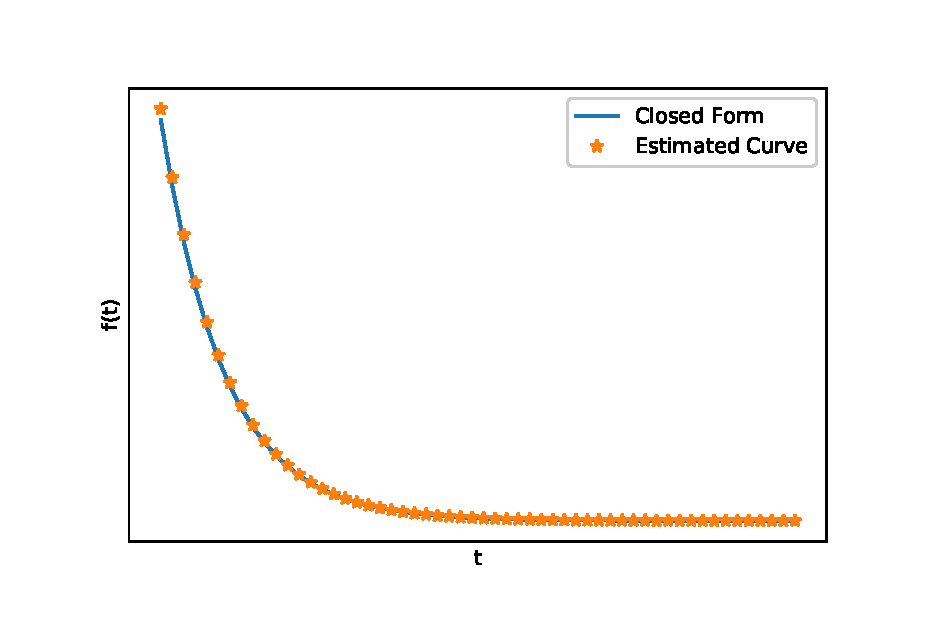
\includegraphics[scale=0.45]{DPMh0091.eps}
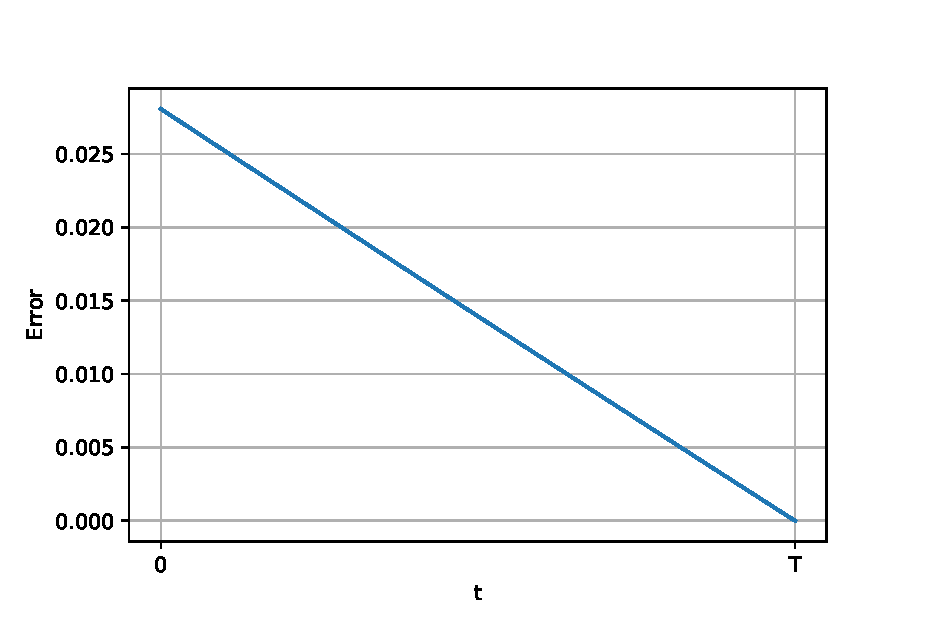
\includegraphics[scale=0.45]{DPMh0091error.eps}
\caption{The curve of $f(t)$ and errors between closed form and the estimated curve $(h=0.091)$}
\label{fig:DPM0091}
\end{figure}
From the figures above, we see that the curve fits well when $h=0.091$, and the error is shown small by the right figure. We define $error=\frac{\text{estimated value}-\text{closed form}}{\text{closed form}}$, so we find the errors are always below $3\%$ in this case. Since we estimate the curve backward, the error, not surprisingly, decreases when $t$ increases.

From common sense, we know that if the step size $h$ is smaller, the curve will be smoother. However, if $h$ is too small, it may lead to bigger errors. This can be shown by comparing the left figure of Figure~\ref{fig:DPM0091} and Figure~\ref{fig:DPM0083}. In these two figures, it is obvious that the estimated cure when $h=0.091$ fits better than the curve when $h=0.083$.
\begin{figure}[H]
\centering
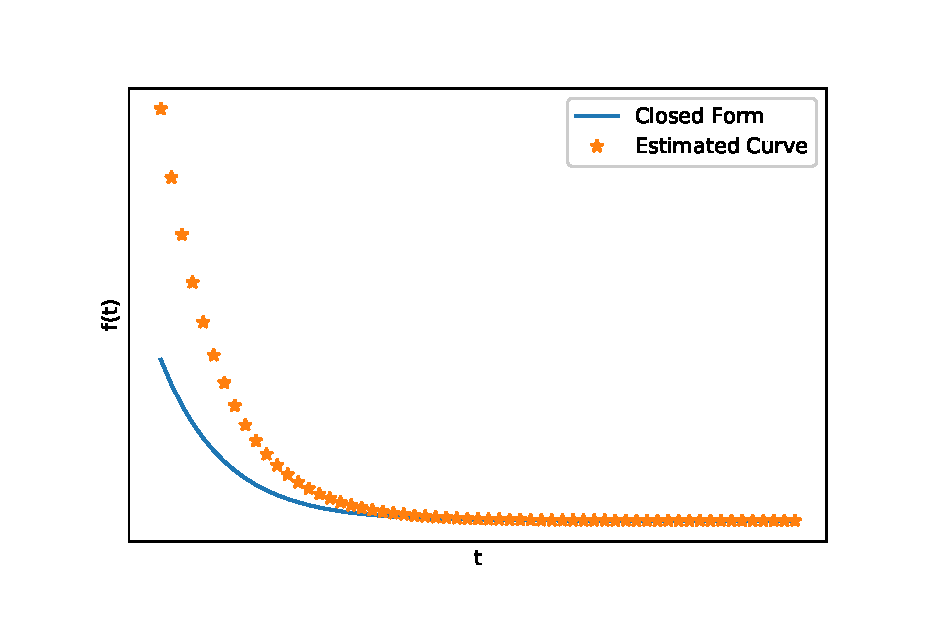
\includegraphics[scale=0.6]{DPMh0083.eps}
\caption{The closed form and the estimated curve of $f(t)$ $(h=0.083)$}
\label{fig:DPM0083}
\end{figure}
In conclusion, we can solve PDEs with boundary condition numerically in almost every cases, but we have to choose the step size $h$ carefully.
\end{exa}

\section{Optimal Consumption Problems}\label{ch:consumption_problem}

In this chapter, we introduce the approach to solve the Merton's consumption problem and the consumption problem with habit formation model. The main difference between consumption problems and terminal wealth problem in the previous chapter is that an investor must not only allocate his wealth between risky and risk-free assets but also decide how much to consume in order to maximize the expected utility of non-negative consumption process $c$. In this chapter, we consider the infinite-horizon problem, thus the objective is maximizing the utility of the consumption process,
\begin{equation}\label{infinity-problem}
u(x)=\max_{\pi_t,c_t}\mathbb E[\int^\infty_0e^{-\rho t}U(c_t)\mathrm dt\lvert X_0=x],
\end{equation}
where $\rho$ represents the discount rate. The greater is $\rho$, the less the individual values future consumption relative to current consumption. Besides, we assume the utility function of this chapter is $U(x)=\frac{1}{\gamma}x^\gamma, \gamma\in(-\infty,1)\setminus\{0\}$.

Note that this is an infinite-horizon problem. In fact, this problem is equivalent to the finite-horizon problem when the stopping time $T\rightarrow\infty$, that is,
\begin{equation}\label{finite-problem}
u(x_0)=\max_{\pi_t,c_t}\mathbb E[\int^T_0e^{-\rho t}U(c_t)\mathrm dt\lvert X_0=x_0],\qquad T\rightarrow\infty.
\end{equation}

Economically speaking, the optimal value function of consumption problems should be negative because the essence of these problems is minimizing the loss of consumption. If the invested wealth is small, the loss would be very huge, while if one invests much, it is predictable that the loss would tend to zero, a very small number.

We consider a financial market with only one risky stock, $S_t$ and one risk-free savings account, $S^0_t$. With the same setting of asset prices in section~\ref{sec:DPM}, the total wealth at time $t$ satisfies
\begin{equation}\label{consumption_SDE}
\begin{aligned}
\mathrm dX_t&=rX_t\mathrm dt+\pi_tX_t(\sigma\mathrm dW_t+(\mu-r)\mathrm dt)-c_t\mathrm dt\\
&=[(r+\pi_t(\mu-r))X_t-c_t]\mathrm dt+\sigma\pi_tX_t\mathrm dW_t,
\end{aligned}
\end{equation}
where $\pi$ denotes the proportion of total wealth to invest in the stock $S$, and the adapted scalar process $c$ represents the consumption stream. This means that there exists a production good, which is also the consumption good, and this good may be consumed or invested in stock and savings account with proportion $\pi$ and $1-\pi$, respectively. Economically speaking, the wealth process and the consumption process should satisfy $X_t>0$ and $c_t\geq0$ for all $t$ almost surely.

\begin{definition}[Admissible~\cite{book3}]
The pair $(\pi_t,c_t)_{t\geq0}$ is said to be \emph{admissible} for initial wealth $x_0$ if the wealth process $X_t$ given by \eqref{consumption_SDE} remains non-negative at all times. We use the notation
$$\mathcal A(x_0)=\{(\pi,c):(\pi,c)\text{ is admissible from initial wealth }x_0\}.$$
We shall write $\mathcal A=\cup_{x>0}\mathcal A(x)$ for the set of all admissible pairs $(\pi,c)$.
\end{definition}

Since the wealth process $X$ should be non-negative, the control variables must be chosen carefully. Here is a principle to ensure the non-negative property of $X$ which is introduced by Rogers (2013)~\cite{book3}.
\begin{theorem}[The Davis-Varaiya Martingale Principle of Optimal Control]\label{th:davis}
Suppose that the objective is \eqref{finite-problem}, and that there exists a function $V:[0,T]\times\mathbb R^+\rightarrow\mathbb R$ which is $C^{1,2}$, such that $V(T,\cdot)=U(T,\cdot)$. Suppose also that
\begin{equation}\label{Ytsupermg}
Y_t:=V(t,x_t)+\int^t_0e^{-\rho s}U(c_s)\mathrm ds\text{ is a supermartingale,}
\end{equation}
and that for some policies $(\pi^*,c^*)$ the process $Y$ is a martingale. Then $(\pi^*,c^*)$ is optimal, and the value of the problem starting from initial wealth $x_0$ is 
$$V(0,x_0)=\sup_{\pi,c}\mathbb E[\int^T_0e^{-\rho t}U(c_t)\mathrm dt\lvert X_0=x_0],\qquad T\rightarrow\infty.$$
\end{theorem}
When $T\rightarrow\infty$, this theorem is suitable for the infinite-horizon problem as well and is used in the each following problems.

\subsection{Merton's Problem}\label{sec:merton}
Merton (1969)~\cite{merton} gave the solution to the problem \eqref{infinity-problem}, and there are many approaches to solve this problem mentioned by Rogers (2013)~\cite{book3}. In this section, we introduce one of those approaches, the value function approach, from~\cite{book3} and numerical method to solve Merton's problem.

With the definition of $Y_t$ in \eqref{Ytsupermg} and Ito expansion, we have
\begin{equation}
\begin{aligned}
\mathrm dY_t&=V_t\mathrm dt+V_x\mathrm dX_t+\frac{1}{2}V_{xx}\mathrm dX_t\mathrm dX_t+e^{-\rho t}U(c)\mathrm dt\\
&=\sigma\pi V_x\mathrm dW_t+\{e^{-\rho t}U(c)+V_t+V_x(rX+\pi X(\mu-r)-c)+\frac{1}{2}\sigma^2\pi^2x^2V_{xx}\}\mathrm dt
\end{aligned}
\end{equation}

With Theorem~\ref{th:davis}, $Y$ should always be a supermartingale whatever $(\pi,c)$ is, so the drift of $Y$ should be non-positive. Additionally, $Y$ should be a martingale for some optimal policies $(\pi,c)$, and then we know $V$ is the value function. Hence we have
\begin{equation}\label{hjb:merton}
0=\sup_{\pi,c}\{e^{-\rho t}U(c)+V_t+V_x(rX+\pi X(\mu-r)-c)+\frac{1}{2}\sigma^2\pi^2x^2V_{xx}\}.
\end{equation}

On the other hand, for the case $U(x)=\frac{1}{\gamma}x^\gamma$, if we consider the value function
\begin{equation}\label{pro:merton}
V(t,x)=\sup_{\pi,c}\mathbb E[\int^\infty_te^{-\rho s}\frac{1}{\gamma}c_s^\gamma\mathrm ds\lvert X_t=x],
\end{equation}
then we have
$$V(t,x)=e^{-\rho t}u(x)$$
because of the time-homgeneity of the problem, where $u(x)$ is defined in \eqref{infinity-problem}.

With this property, we get
\begin{equation}\label{hjb:merton2}
0=\sup_{\pi,c}e^{-\rho t}\{U(c)-\rho u+u_x(rx+\pi x(\mu-r)-c)+\frac{1}{2}\sigma^2\pi^2x^2u_{xx}\}.
\end{equation}
Then taking the derivative with respect to $\pi$ and $c$, we have
\begin{equation}\label{piandc}
\hat\pi(x)=-\frac{\mu-r}{\sigma^2}\frac{u_x}{xu_{xx}}\text{, and }
\hat c(x)=u_x^\frac{1}{\gamma-1}.
\end{equation}
Hence we obtain the HJB equation for $u(x)$
\begin{equation}\label{hjb:merton3}
\frac{1-\gamma}{\gamma}u_x^\frac{\gamma}{\gamma-1}-\rho u+rxu_x-\frac{(\mu-r)^2}{2\sigma^2}\frac{u_x^2}{u_{xx}}=0.
\end{equation}

Rogers (2013)~\cite{book3} also showed an important property of the optimal value function as following.
\begin{proposition}[Scaling~\cite{book3}]
Suppose that the problem \eqref{pro:merton} is well posed. Then the value function takes the form
$$u(x)=\gamma_M^{\gamma-1}U(x)=\gamma_M^{\gamma-1}\frac{1}{\gamma}x^\gamma.$$
\end{proposition}
\begin{proof}
By the linearity of the wealth equation \eqref{DPM_SDE}, it is clear that
$$(\pi,c)\in\mathcal A(x)\Leftrightarrow(\lambda\pi,\lambda c)\in\mathcal A(\lambda x)$$
for any $\lambda>0$. Hence
\begin{equation}
\begin{aligned}
V(\lambda x)&=\sup_{(\pi,c)\in\mathcal A(\lambda x)}\mathbb E[\int^\infty_0e^{-\rho t}U(c_t)\mathrm dt]\\
&=\sup_{(\pi,c)\in\mathcal A(x)}\mathbb E[\int^\infty_0e^{-\rho t}U(\lambda c_t)\mathrm dt]\\
&=\sup_{(\pi,c)\in\mathcal A(x)}\lambda^\gamma\mathbb E[\int^\infty_0e^{-\rho t}U(c_t)\mathrm dt]\\
&=\lambda^\gamma V(x).
\end{aligned}
\end{equation}
\end{proof}
Then, substituting this into the HJB equation \eqref{hjb:merton3}, we can obtain
$$\gamma_M=\frac{1}{1-\gamma}[\rho-\gamma(r+\frac{(\mu-r)^2}{2\sigma^2(1-\gamma)})],$$
so the closed form of $u(x)$ is obtained now and with \eqref{piandc}, we have
\begin{equation}
\begin{aligned}
&\hat c_t=\gamma_Mx_t\\
&\hat\pi_t=\frac{\mu-r}{(1-\gamma)\sigma^2}.
\end{aligned}
\end{equation}

\subsubsection{Numerical Method}
Now we are going to show detailedly how numerical method works, which is suitable for most HJB equations, including those who do not have a closed form. The parameters in this chapter are
$$\gamma=-1,\rho=0.02,\sigma=0.35,r=0.05,\mu=0.14.$$

Before we do programming, the HJB equation \eqref{hjb:merton3} can be deduced by hand, and the boundary conditions should be considered. In fact, for an infinite-horizon problem, we do not have boundary conditions to fix a solution. However, economically speaking, the curve of $u(x)$ should be convergent and close to zero in this case when $x$ is big enough. Hence what we should do next is to solve the ODE
\begin{equation}\label{ode:merton}
\left\{
\begin{aligned}
&\frac{1-\gamma}{\gamma}u_x^\frac{\gamma}{\gamma-1}-\rho u+rxu_x-\frac{(\mu-r)^2}{2\sigma^2}\frac{u_x^2}{u_{xx}}=0\\
&u(500)=-1\\
&u_x(500)=0.02.
\end{aligned}
\right.
\end{equation}

First, since $x>0$, we set $x\in[0.01,500]$ and divide this interval into $N$ parts such that the step size $h$ is a small number, e.g $h=10^{-6}$.

Then we rewrite the first equation of ODE as
$$u_{xx}=\frac{\frac{(\mu-r)^2}{2\sigma^2}u_x^2}{\frac{1-\gamma}{\gamma}u_x^\frac{\gamma}{\gamma-1}-\rho u+rxu_x}=:f(x,u,u_x).$$

Suppose $y=u_x=u'$, then $y'=u_{xx}$.
With the finite-difference method and Taylor extension, for each interval $[x_{i-1},x_i]$, we have
\begin{equation}\label{fdm:merton}
\left\{
\begin{aligned}
&y_{i-1}=y_i-hf(x_i,u_i,y_i),\qquad i=1,2,\dots,N\\
&u_{i-1}=u_i-hy_i+\frac{1}{2}h^2f(x_i,u_i,y_i).
\end{aligned}
\right.
\end{equation}

Since we know the terminal conditions of this curve, we work backwards. At the end point, i.e, $i=N$, $u_N$ and $y_N$ are available from \eqref{ode:merton}. Then $u_{N-1}$ and $y_{N-1}$ can be calculated by \eqref{fdm:merton}. Repeating computing \eqref{fdm:merton} until $i=1$, we have the points $u_N,u_{N-1},\dots,u_0$, and the curve is drawn as the following figure shows.
\begin{figure}[H]
\centering
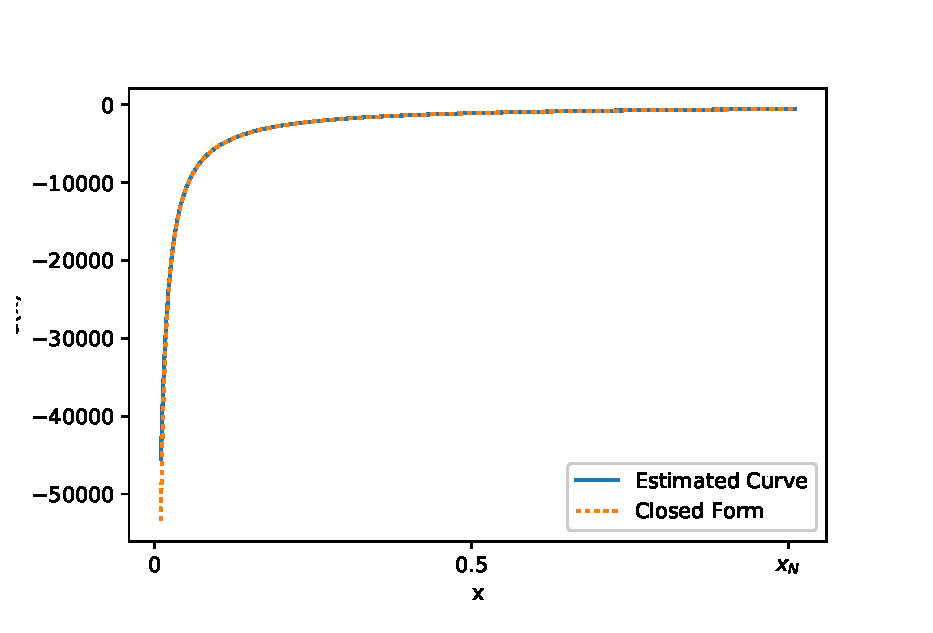
\includegraphics[scale=0.6]{MertonV.eps}
\caption{The estimated and closed-form curves of $u(x)$ against $x$}
\label{fig:Merton}
\end{figure}

The curves in Figure~\ref{fig:Merton} is obtained when the step size $h=10^{-6}$, and it seems that that the finite-difference method applied in this problem fits its closed form well, both curves of which show the properties of $u(x)$ of Merton's problem. It is obvious that $u(x)$ tends to $-\infty$ when $x$ is close to zero, and seems to converge early, even before $x=0.5$. Furthermore, the function has an extremely sharp increasing trend at first, and suddenly changes to a slight increase at a certain point around $x=0.1$. This implies that in Merton's problem, if an investor holds only a little initial wealth in hand, he must lose much on consumption good, even if he invests optimally, but if he invests a bit more money on it, he may have much less loss. Conversely, once he invests enough money on this consumption product, his optimal expected utility function of consumption seems to converge to zero, which represents a very small loss.

\begin{figure}[H]
\centering
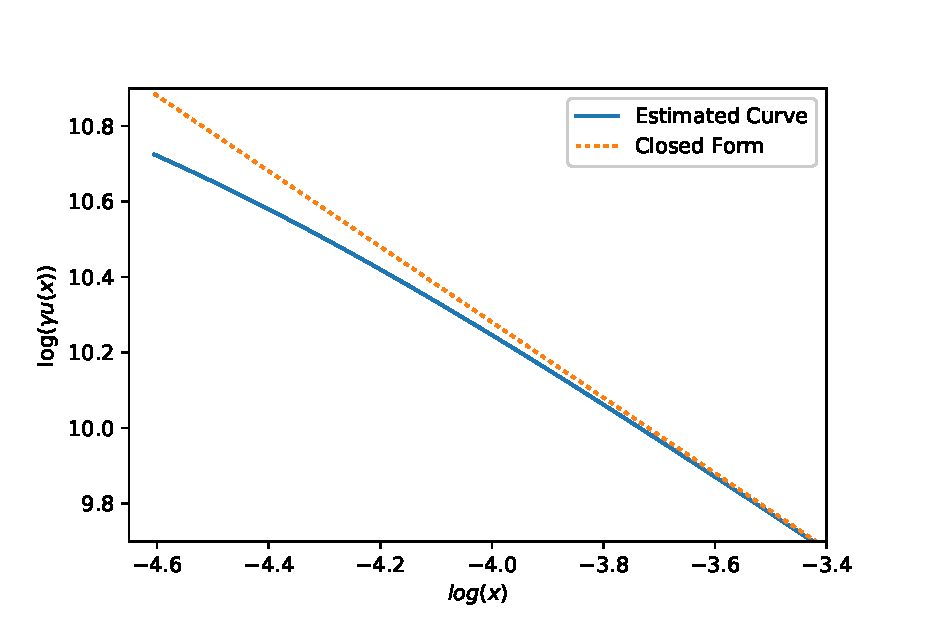
\includegraphics[scale=0.45]{MertonVlog.eps}
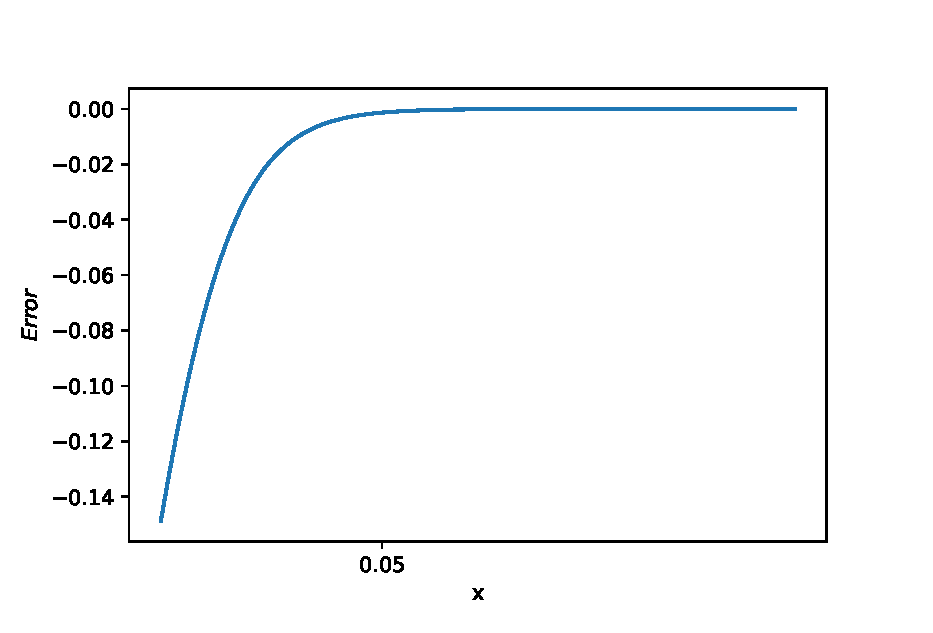
\includegraphics[scale=0.45]{MertonVerror.eps}
\caption{The curves of $\log(\gamma u(x))$ against $\log(x)$ and error between closed form and estimated curve}
\label{fig:MertonError}
\end{figure}
In fact, the error is not so apparent in Figure~\ref{fig:Merton} that we enlarge them in Figure~\ref{fig:MertonError}. We transform $x$ and $u(x)$ into $\log(x)$ and $\log(\gamma u(x))$ to show errors graphically in the left figure, and calculate $\text{error}=\frac{\text{estimated value}-\text{closed form}}{\text{closed form}}$ to show errors numerically in the right figure. It is predictable that error decreases with $x$ increasing because we estimated this curve backward. Therefore not surprisingly, we can see that the errors become visibly if $x<e^{-3.8}$, approximately $0.022$. On the other figure, error becomes larger when $x<0.05$, and the biggest error is less than $16\%$. Hence we can conclude that the finitedifference method is effective for this case and fits the closed form well.

With these $N$ points of $u(x)$, the optimal trading strategies $\hat\pi(x)$ and $\hat c(x)$ can be obtained by
$$\hat\pi_i=-\frac{\mu-r}{\sigma^2}\frac{y_i/x_i}{f(x_i,u_i,y_i)}\text{, and }
\hat c_i=y_i^\frac{1}{\gamma-1},$$
and the results are shown in Figure~\ref{fig:MertonPi} and Figure~\ref{fig:MertonC}.
\begin{figure}[H]
\centering
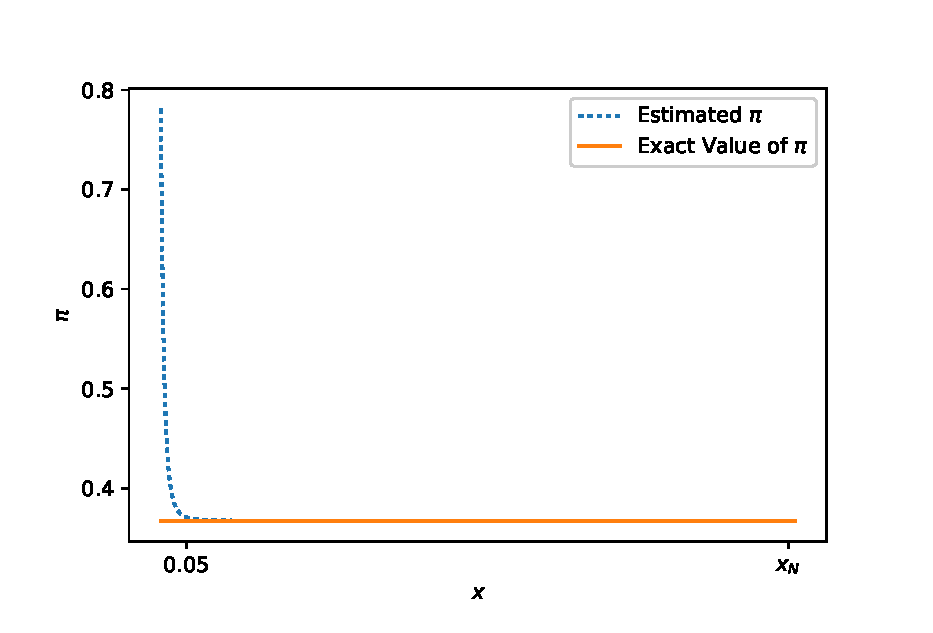
\includegraphics[scale=0.45]{Mertonpi.eps}
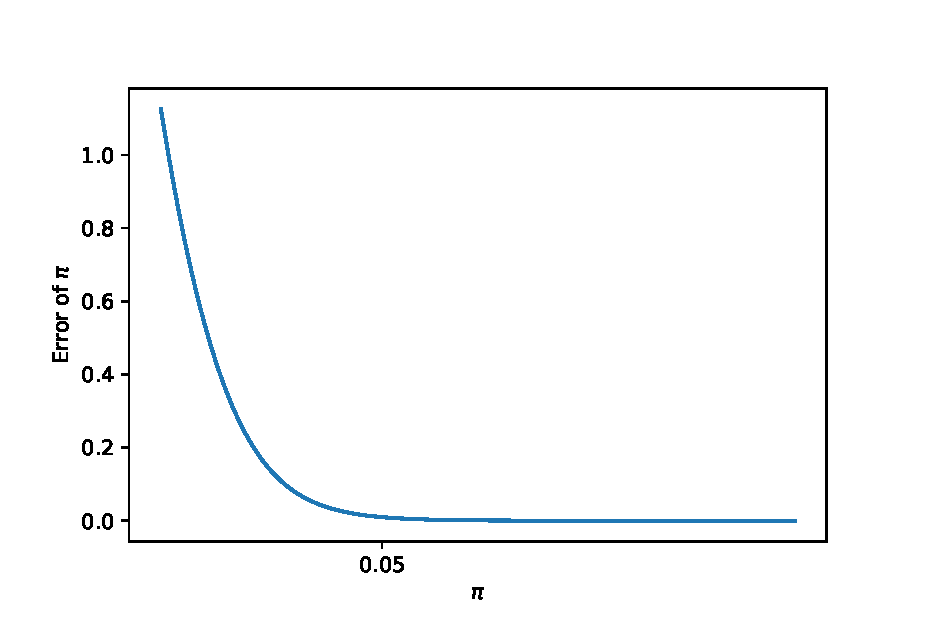
\includegraphics[scale=0.45]{Mertonpierror.eps}
\caption{The curves of $\hat\pi(x)$ in the left and error in the right}
\label{fig:MertonPi}
\end{figure}
\begin{figure}[H]
\centering
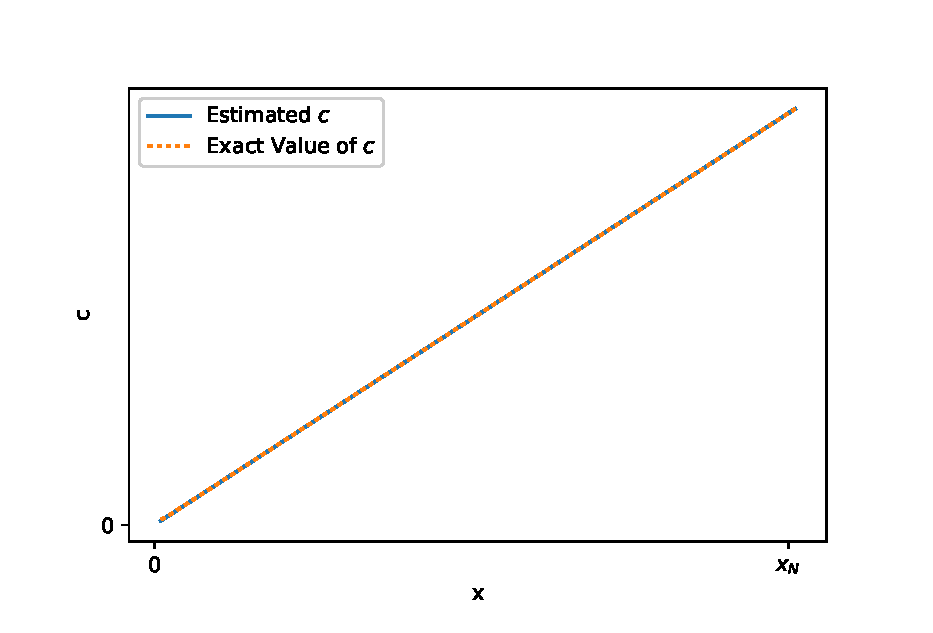
\includegraphics[scale=0.45]{Mertonc.eps}
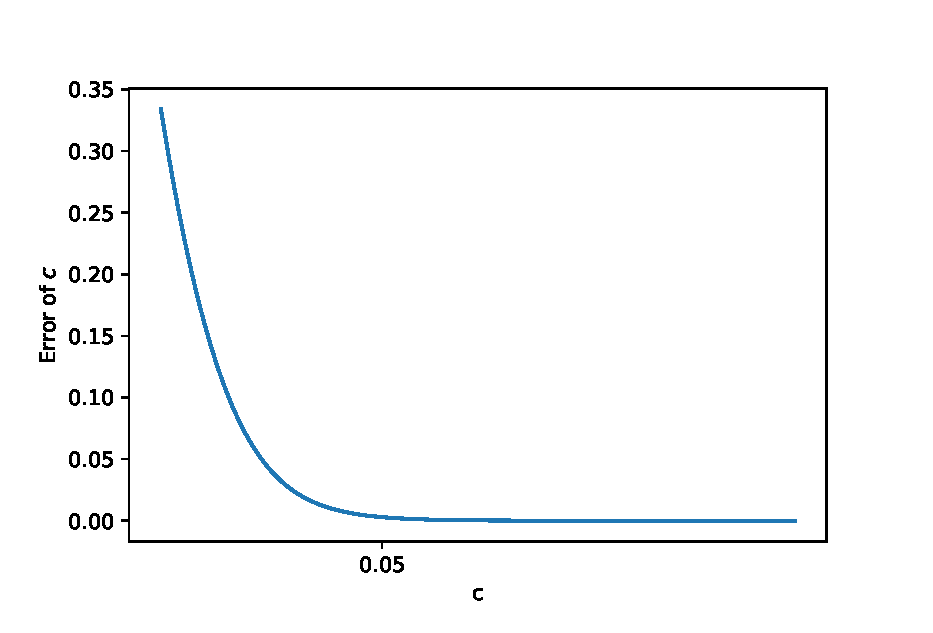
\includegraphics[scale=0.45]{Mertoncerror.eps}
\caption{The curves of $\hat c(x)$ in the left and error in the right}
\label{fig:MertonC}
\end{figure}

From the figures above, the optimal trading strategy of the stock is constant no matter how much initial wealth $x$ invested, and the optimal consumption stream is proportional to $x$. For errors, we find unsurprisingly that the errors of $u(x)$, $\hat\pi(x)$ and $\hat c(x)$ are all big before a certain wealth, 0.05.

\subsection{Habit Formation Model}
After the Merton's problem, let us discuss a more general case.
The habit formation model is a model where the investor's present consumption is related to an exponentially-weighted historical average of past consumption, $\overline c$.
Therefore in this model, we assume that
$$\mathrm d\overline c_t=bc_t\mathrm dt-a\overline c_t\mathrm dt.$$
This implies
$$\overline c_t=e^{-at}\overline c_0+b\int^t_0e^{a(s-t)}c_s\mathrm ds.$$
If $a=b=0$, there is no habit formation model, and the problems reduce to the Merton's problem as introduced in the previous section. If the parameter $a$ becomes larger, then less weight is given to past consumption in determining $\overline c_t$. If $b$ is larger, then the less weight is given to habit formation among it. That is, the parameter $b$ measures the strength of habit formation, with positive values of $b$ implying habit formation.

Constantinides (1990)~\cite{constantinides} solved the infinite-horizon problem
$$u(x_0,\overline c_0)=\max_{\pi_t,c_t}\mathbb E[\int^\infty_0e^{-\rho t}U(c_t,\overline c_t)\mathrm dt\lvert X_0=x_0]$$
where $U(c_t,\overline c_t)=\frac{(c_t-\overline c_t)^\gamma}{\gamma}$, %Note that the case $\gamma=0$ corresponds to logarithmic utility and may be treated differently.
\iffalse
The common objectives of consumption-investment problems  are finite-horizon problem
$$\max_{\pi_t,c_t}\mathbb E[\int^T_0U_1(t,c_t)\mathrm dt+U_2(T,X_T)],$$
and infinite-horizon problem
$$\max_{\pi_t,c_t}\mathbb E[\int^\infty_0U(t,c_t)\mathrm dt]$$
with initial wealth $x$.
The utility function $U$ is assumed to satisfy the Assumption~\ref{usual conditions}.
\fi
while Xiao and Xu (2003)~\cite{c-i with wealth} extended his model and considered a model in which a investor's preference depends on not only the consumption history but also the preference for wealth. Hence the utility function is
\begin{equation}\label{problem with wealth2}
U(c_t,X_t,\overline c_t)=\frac{1}{\gamma}(c_t-\overline c_t+\lambda X_t)^\gamma,
\end{equation}
and we aim to solve the consumption with this utility function by both value function method and numerical method in this section.
If $\lambda=0$, this problem reduces to the problem with habit formation model by Constantinides (1990)~\cite{constantinides}.

Since $U(c_t,X_t,\overline c_t)$ is a function of three variables, the usual regularity conditions of utility function should be extended.

\begin{assumption}
The utility function $U(c_t,X_t,\overline c_t)$ is twice continuously differentiable, $U_c>0$, $U_x>0$, $U_{\overline c}>0$ and $U_{cc}$, $U_{xx}$, $U_{\overline c\overline c}>0$.
\end{assumption}

To solve this case, we first define the value function
$$V(x,\overline c)=\max_{\pi_s,c_s}\mathbb E[\int^\infty_te^{-\rho(s-t)}\frac{1}{\gamma}(c_s-\overline c_s+\lambda X_s)^\gamma\mathrm ds\lvert X_t=x,\overline c],$$
and we aim to obtain this function at $t=0$.
%Then, our objective is to find the function $$V(x,\overline c)=\max_{\pi_s,c_s}\mathbb E[\int^\infty_0e^{-\rho t}\frac{(c_t-\overline c_t+\lambda X_t)^\gamma}{\gamma}\mathrm dt\lvert X_0=x,\overline c_0=\overline c].$$

Similar to the Section~\ref{sec:merton}, by Theorem~\ref{th:davis}, we have the HJB equation
\begin{equation}\label{hf1suphjb}
0=\sup_{\pi,c}e^{-\rho t}(U-\rho V+\{[(\mu-r)\pi+r]x-c\}V_x+\frac{\pi^2\sigma^2}{2}x^2V_{xx}+(bc-a\overline c)V_{\overline c}).
\end{equation}

Then, taking the derivative with respect to $\pi,c$, we obtain
\begin{equation}\label{hf1optimalpic}
\begin{aligned}
U_c(c^*,x,\overline c)=V_x-bV_{\overline c}\\
\pi^*=-\frac{\mu-r}{\sigma^2}\frac{V_x}{xV_{xx}}
\end{aligned}
\end{equation}

Substituting \eqref{hf1optimalpic} into \eqref{hf1suphjb}, we get
\begin{equation}\label{hf1hjb}
0=\frac{1-\gamma}{\gamma}(V_x-bV_{\overline c})^\frac{\gamma}{\gamma-1}-\rho V+(rx-\overline c)V_x+(b-a)\overline cV_{\overline c}-\lambda x(V_x-bV_{\overline c})-\frac{(\mu-r)^2}{2\sigma^2}\frac{V_x^2}{V_{xx}}
\end{equation}

To solve this ODE, we conjecture that the value function has the form $V(x,\overline c)=g(x-k\overline c)^\gamma$, and by substituting it into \eqref{hf1optimalpic}, we get
\begin{equation}\label{HF_c_optimal}
c^*=\overline c+h(x-k\overline c)-\lambda x
\end{equation}
\begin{equation}\label{HF_pi_optimal}
\pi^*=\frac{\mu-r}{(1-\gamma)\sigma^2}\frac{x-k\overline c}{x},
\end{equation}
where $h=\big(g\gamma(1+kb)\big)^\frac{1}{\gamma-1}>\lambda$. Then $g,k$ can be obtained by substituting these into \eqref{hf1hjb}.

Xiao and Xu (2003)~\cite{c-i with wealth} gave the results of this problem as well, but we think there are some assumptions necessary but missing in their paper.

First of all, as mentioned at the beginning of this chapter, the consumption stream $c_t$ must be non-negative, so by equation \eqref{HF_c_optimal}, conditions $\overline c_0\geq0$, $h>\lambda$ and $x_t-k\overline c_t$ must be satisfied. Note that if $x_0>k\overline c_0$, then $x_t-k\overline c_t$ satisfies log-normal distribution with a state space of $(0,\infty)$. Hence with the condition $x_t>k\overline c_t$, the value function makes economic sense, and this condition can be replaced by $x_0>k\overline c_0$.
Secondly, to make sure the condition $0\leq\pi_t\leq1$ of an admissible policy is non-binding, by equation \eqref{HF_pi_optimal}, we assume $0\leq\frac{\mu-r}{(1-\gamma)\sigma^2}\leq1$.
Then the optimal consumption and control are at an interior maximum, and this simplification leads to closed-form expressions.

Additionally, condition $g<0$ ensures that, under the optimal policies, the expected utility of consumption flow grows at a rate that is lower than the time preference so that the expected utility of consumption over the infinite horizon is finite. It also implies that the appropriate transversality condition is satisfied.

Finally, we summarize the results in the following theorem.
\begin{theorem}\label{th:wealth}
To make sure that there exists a unique optimal policy and closed form, the following conditions should be satisfied.
$$x_0>0,\quad\overline c_0\geq0,\quad x_0-k\overline c_0>0,$$
$$0\leq\frac{\mu-r}{(1-\gamma)\sigma^2}\leq1$$
$$0<b<r+a,$$
$$\rho-\gamma r-\frac{\gamma(\mu-r)^2}{2(1-\gamma)\sigma^2}-\gamma\lambda\frac{r+a}{r+a-b+\lambda b^2}>0.$$
Then, the optimal consumption and portfolio policy can be written as
$$c^*=\overline c+h(x-k\overline c)-\lambda x$$
$$\pi^*=\frac{\mu-r}{(1-\gamma)\sigma^2}\frac{x-k\overline c}{x}$$
and the indirect utility function is 
$$V(x,\overline c)=g(x-k\overline c)^\gamma,$$
where
$$k=\frac{1-\lambda b}{r+a-b+\lambda b^2},\qquad h=\big(g\gamma(1+kb)\big)^\frac{1}{\gamma-1}>\lambda,$$
$$g=\frac{(1-\gamma)^{1-\gamma}}{\gamma}\Big(\frac{r+a}{r+a-b+\lambda b^2}\Big)^{-\gamma}\Big[\rho-\gamma r-\frac{\gamma(\mu-r)^2}{2(1-\gamma)\sigma^2}-\gamma\lambda\frac{r+a}{r+a-b+\lambda b^2}\Big]^{\gamma-1}.$$
\end{theorem}
This theorem is consistent with the result by Constantinides (1990)~\cite{constantinides} in the case of $\lambda=0$.

\iffalse
\subsection{Maximizing the Expected Utility not Depending on $X_t$}
Now we discuss a more special case, letting $\lambda=0$ in the section~\ref{problemwithwealth}, then the utility function becomes
$$U(c_t,\overline c_t)=\frac{(c_t-\overline c_t)^\gamma}{\gamma},$$
and the objective is
$$V(x_t,\overline c_t)=\max_{\pi_s,c_s}\mathbb E[\int^\infty_te^{-\rho(s-t)}\frac{(c_s-\overline c_s)^\gamma}{\gamma}\mathrm ds\lvert X_t=x_t,\overline c_t],$$
where $\gamma<1$ and $\gamma\neq0$.

This utility function has the property that as $c_t\rightarrow\overline c_t$, the marginal utility tends to $\infty$. So the level $\overline c_t$ serves as a natural "floor level of consumption" below which the investor will never allow the consumption rate to fall.

With this model, Constantinides\cite{constantinides} solved this consumption-investment problem and conclude the following theorem, which corresponds to the case $\lambda=0$ of Theorem~\ref{thwealth}.
\begin{theorem}
In the model described above, an optimal admissible consumption and investment policy exists, is unique, and is given by
$$c_t^*=\overline c_t+h[X_t-\frac{\overline c_t}{r+a-b}]$$
and
$$\pi^*_t=m\big[1-\frac{\overline c_t}{(r+a-b)x_t}\big],$$
where $h=[\frac{r+a-b}{(r+a)(1-\gamma)}][\rho-\gamma r-\frac{\gamma(\mu-r)^2}{2(1-\gamma)\sigma^2}]>0$, and $m=\frac{\mu-r}{(1-\gamma)\sigma^2}$.

The derived utility of capital is
$$V(x_t,\overline c_t)=\frac{(r+a-b)h^{\gamma-1}}{(r+a)\gamma}\big[x_t-\frac{\overline c_t}{r+a-b}\big]^\gamma.$$
\iffalse
The capital is
$$X_t=\frac{\overline c_t}{r+a-b}+\bigg(X_0-\frac{\overline c_0}{r+a-b}\exp{\Big[\big(n-\frac{m^2\sigma^2}{2}\big)t+m\sigma W_t\Big]}\bigg)$$
where $n=\frac{r-\rho}{1-\gamma}+\frac{(\mu-r)^2(2-\gamma)}{2(1-\gamma)^2\sigma^2}$
\fi
\end{theorem}
\fi
The function $V(x,\overline c)$ is shown in the following figures. To make the 3D graph visible, we fix $\overline c$ as 0,24 and 48, and show the curves of $V(x,.)$ in the left figure, while the initial wealth $x$ is fixed and $V(.,\overline c)$ are plotted when $x=100,300$ and $500$ in the right figure. The points in x-axis, $x1,x2,x3$ and $c1,c2,c3$, represent the extreme points which satisfy $x-k\overline c>0$. We can see that $V(x,\overline c)$ tends to negative infinite when $x-k\overline c$ tends to zero, and $V(x,\overline c)$ tends to zero when $x$ tends to infinite and $\overline c$ tends to zero. In fact, the curve in the case of $C=0$ in the left figure is the same as the value function of Merton's problem.
\begin{figure}[H]
\centering
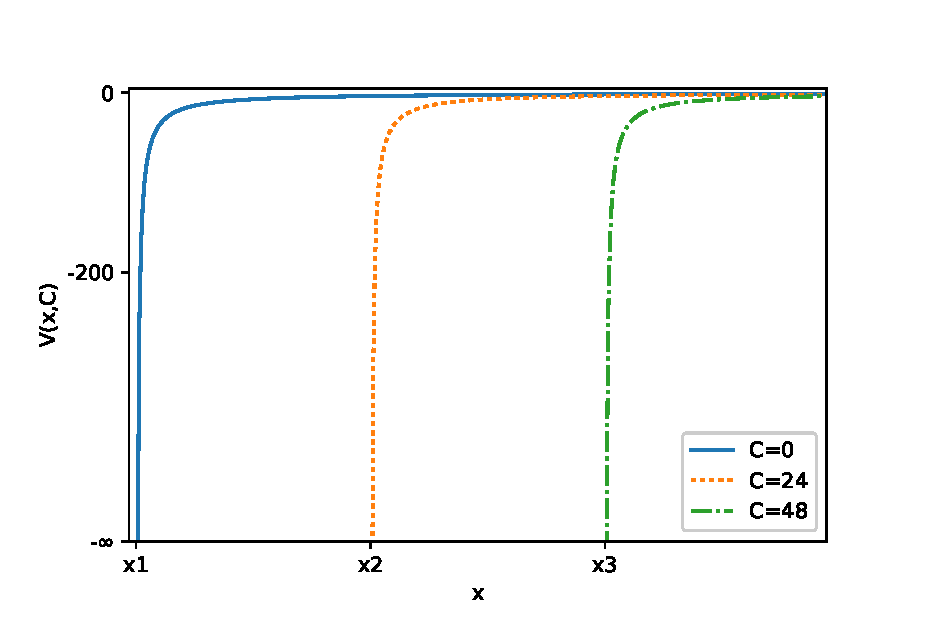
\includegraphics[scale=0.45]{HFcompareVx.eps}
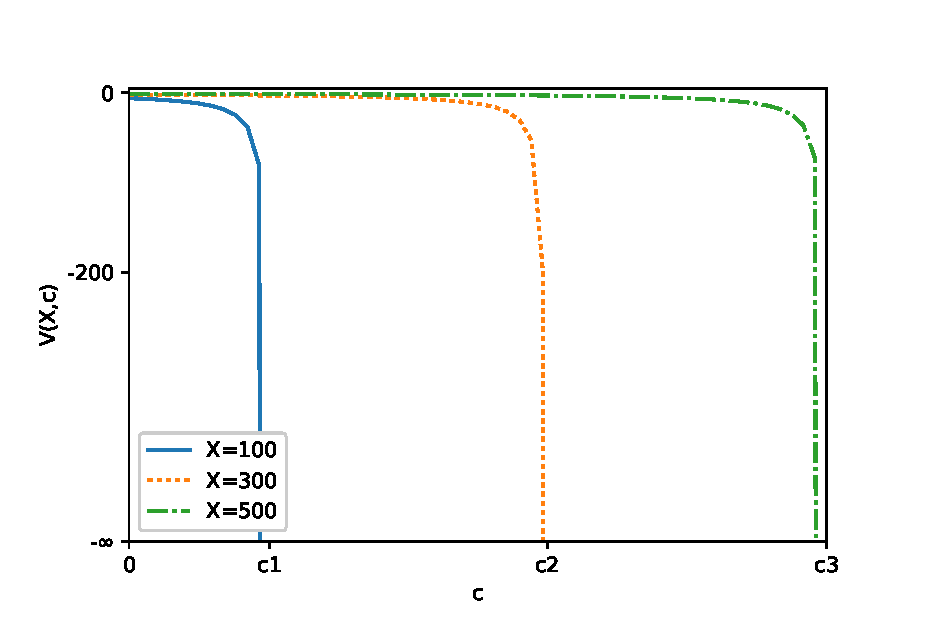
\includegraphics[scale=0.45]{HFcompareVc.eps}
\caption{Curves of $V(x,\overline c)$}
\label{fig:CompareV}
\end{figure}

\subsubsection{Numerical Method}
Similar to the Merton's problem, we can use the finite difference method to solve the PDE \eqref{hf1hjb}. However, it is much more complex because the function $V(x,\overline c)$ has two variables.

We divide the intervals of $x$ and $\overline c$ into $N_x$ and $N_{\overline c}$ parts respectively. Note that $x$ starts at a small number instead of zero, while $\overline c$ starts from zero because of the assumptions in Theorem~\ref{th:wealth} to make economic sense.

With the value function of Merton's problem, which is equivalent to this problem when $\overline c=0$, we know that $V(x,0)$ converges if $x$ is large enough. Therefore when we set $x_{N_x}$ be a large number, we assume 
$V(x_{N_x},\overline c_0)=V^{Merton}(x_{N_x})$, and $V_x(x_{N_x},\overline c_0)=V^{Merton}_x(x_{N_x})$. Furthermore, no matter what $\overline c$ is, $V_x(x_{N_x},.)$ should tend to zero, so we assume $V_x(x_{N_x},.)$ to be same as $V_x(x_{N_x},\overline c_0)$. Besides, $V_{\overline c}(x_{N_x},\overline c_0)$ is assumed to be a negative number close to zero because the value function should decrease in $\overline c$ and converge as well if the exponentially-weighted historical average of past consumption, $\overline c$, tends to zero. Hence we have boundary conditions $V(x_{N_x},\overline c_0),V_x(x_{N_x},.)$ and $V_{\overline c}(x_{N_x},\overline c_0)$ now.

Next, the equation \eqref{hf1hjb} can be written as
$$V_{xx}=\frac{\frac{(\mu-r)^2}{2\sigma^2}V_x^2}{\frac{1-\gamma}{\gamma}(V_x-bV_{\overline c})^\frac{\gamma}{\gamma-1}-\rho V+(rx-\overline c)V_x+(b-a)\overline cV_{\overline c}-\lambda x(V_x-bV_{\overline c})}=:f(x,\overline c,V_x,V_{\overline c},V).$$

We set $y^x=V_x$, $y^{\overline c}=V_{\overline c}$, so for each interval $[i-1,i]$ or $[j,j+1]$, we then have
\begin{equation}\nonumber
\left\{
\begin{aligned}
&y^x_{i-1}=y^x_i-hf(x_i,\overline c_j,y^x_i,y^{\overline c}_j,V_{i,j})\\
&V_{i-1,j}=V_{i,j}-hy^x_i+\frac{1}{2}h^2f(x_i,\overline c_j,y^x_i,y^{\overline c}_j,V_{i,j})\\
&V_{i,j+1}=V_{i,j}+hy^{\overline c}_i\\
&y^{\overline c}_{j+1}=\frac{V_{N_x,j+1}-V_{N_x,j}}{h},
\end{aligned}
\right.
\end{equation}
where $i=0,1,\dots,N_x$ and $j=0,1,\dots,N_{\overline c}$.

To obtain the values of $V_{i,j}$, we do an external loop for $j$ from $0$ to $N_{\overline c}+1$ and an internal loop for $i$ from $N_x$ to $1$. Note that if $x_i-k\overline c_j\leq0$, it does not make economic sense, so we set $V_{i,j}$ a number close to $-\infty$.

\iffalse
\begin{figure}[H]
\centering
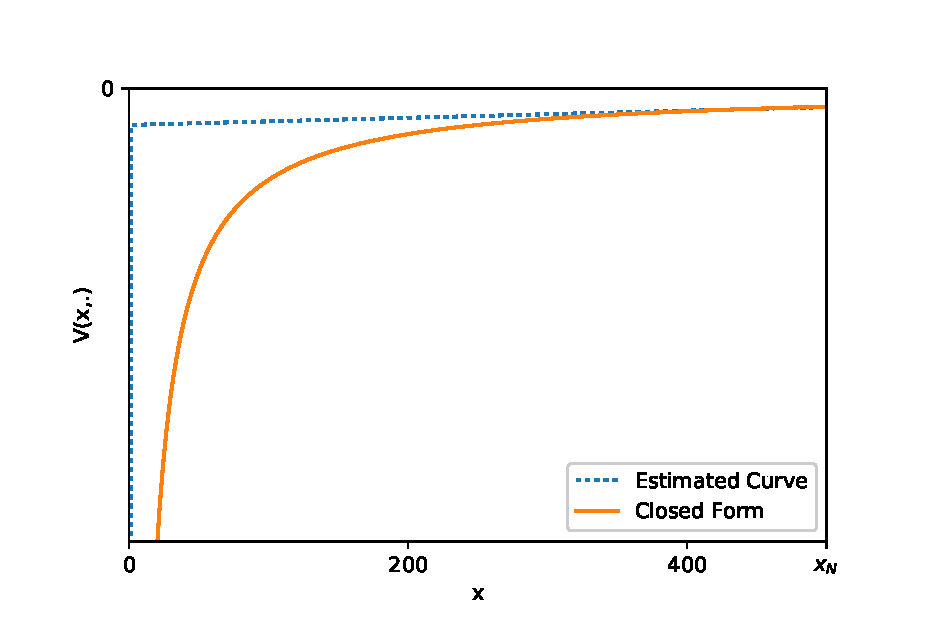
\includegraphics[scale=0.45]{HFVx.eps}
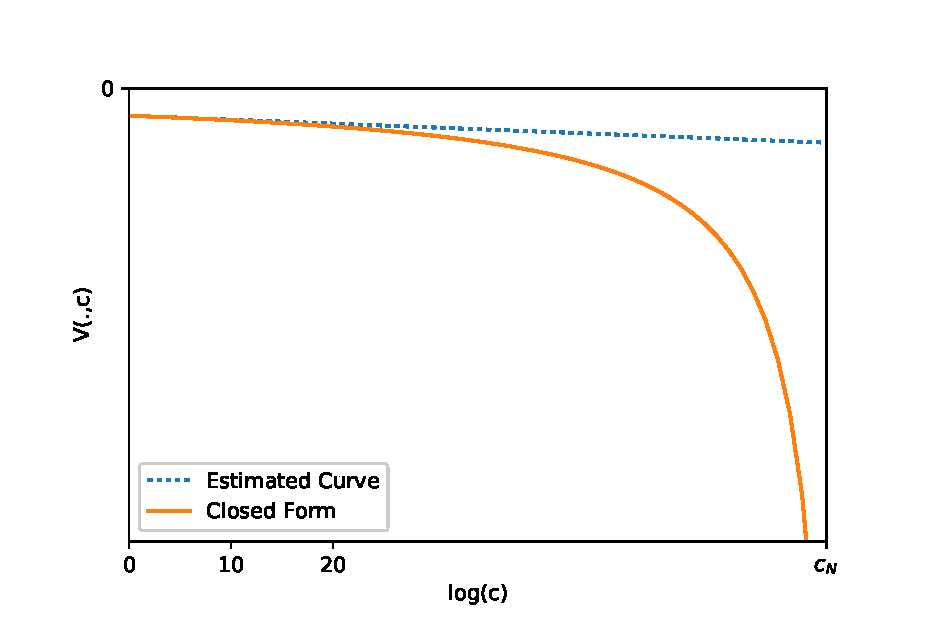
\includegraphics[scale=0.45]{HFVc.eps}
\caption{Curves of $V$}
\label{fig:HFV}
\end{figure}
\fi

Finally, the errors between the estimated values of $V_{i,j}$ and the closed form are shown below. Note that there are some null data, which do not make economic sense because they fail to satisfy $x_i-k\overline c_j\leq0$.
\begin{table}[H]
\centering
\begin{tabular}{c|cccccc }
\hline
& $c_0$ & $c_{0.2N_c}$ & $c_{0.4N_c}$ & $c_{0.6N_c}$ & $c_{0.8N_c}$ & $c_{N_c}$\\
\hline			
$x_{0.2N_x}$ & 0.6410 & 0.9751 & / & / & / & / \\
$x_{0.4N_x}$ & 0.3616 & 0.6206 & 0.9504 & / & / & / \\
$x_{0.6N_x}$ & 0.1616 & 0.3456 & 0.6004 & 0.9260 & / & / \\
$x_{0.8N_x}$ & 0.0411 & 0.1501 & 0.3299 & 0.5804 & 0.9018 & / \\
$x_{N_x}$ & 0.00001 & 0.0340 & 0.1377 & 0.3143 & 0.5607 & 0.8779 \\
\hline  
\end{tabular}
\caption{Errors}
\end{table}
From the table above, we can image that the curve fits worse when point $(x_i,\overline c_j)$ becomes far from $(x_{N_x},\overline c_0)$, but most of the errors are acceptable. Hence we conclude again that the finite difference method is still useful in this case.

\subsection{Comparison with Merton's Problem and Habit Formation Model}
As mentioned in the last section, Merton's problem is a special case of the consumption problem with the habit formation model because if we consider $a=b=0$, the history consumption term disappears in habit formation model. Therefore these two problems can be compared to find the differences of the optimal policies with and without the knowledge of history consumption.

After setting appropriate parameters and fixing $\overline c_t$, we draw the optimal $c_t$ and $\pi_t$ against $x$ in Figure~\ref{fig:CompareC} and Figure~\ref{fig:ComparePi}. Both two figures compare the problem \eqref{problem with wealth2} with different $\lambda$ and Merton's problem. The case of $\lambda=0$ represents Constantinides's problem.

The points in x-axis  of the following two figures, x1, x2 and x\_min, represent the minimum wealths of the cases with different $\lambda$ such that $x_t>k\overline c_t$.
%Next, we compare $c_t^*$ and $\pi_t^*$ in the case with and without the $\overline c_t$ term.
%In this section, we set the parameters as follows: $$\gamma=-1,\quad\rho=0.02,\quad\sigma=0.35,\quad r=0.05,\quad\mu=0.14,\quad a=b=1.$$
\begin{figure}[H]
\centering
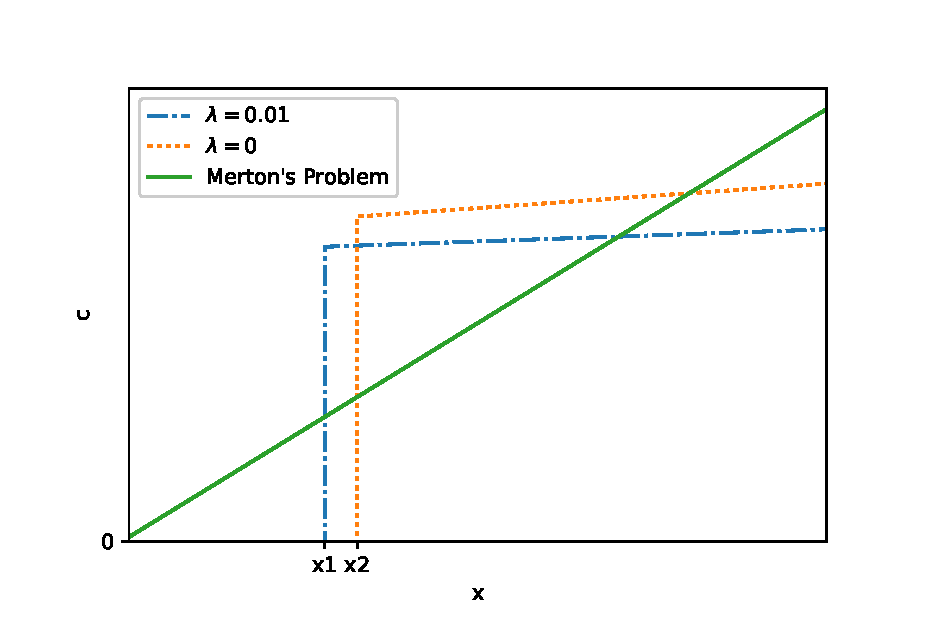
\includegraphics[scale=0.6]{Comparec.eps}
\caption{Comparison of $c^*_t(x_t)$}
\label{fig:CompareC}
\end{figure}
In Figure~\ref{fig:CompareC}, it is obvious that the optimal consumption policy is increasing in wealth no matter for Merton's problem or problem with habit formation model. However, the function for habit formation model increases more slowly than Merton's problem, and there exists an intersection between habit formation problem and Merton's problem. This implies that when the wealth $x_t$ is greater than a certain value, an investor may optimally consume more without considering the past consumption. On the other hand, we can see from this figure that a greater $\lambda$ leads to a more slight increase. 
\begin{figure}[H]
\centering
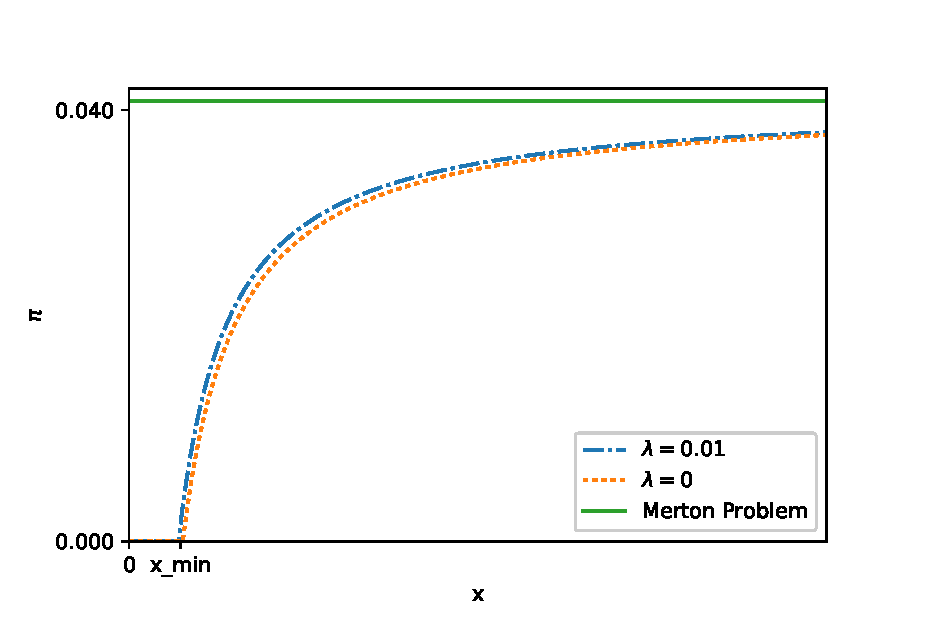
\includegraphics[scale=0.6]{Comparepi.eps}
\caption{Comparison of $\pi^*_t(x_t)$}
\label{fig:ComparePi}
\end{figure}
Figure~\ref{fig:ComparePi} shows that the fraction of wealth invested in the risky asset, $\pi$, is a constant for Merton's problem, while it becomes an increasing concave function of wealth in the problem with habit formation model. Besides, the curves with different $\lambda$ are always below and asymptotically approach the value of $\pi$ in Merton's problem. Additionally, a bigger $\lambda$ results in a greater optimal proportion of wealth to invest in the risky asset.

\iffalse
\subsection{A Model with Hyperbolic Discounting}
main reference: [Optimal Consumption and Investment with Habit Formation and Hyperbolic discounting]

Model:
$$\mathrm dX_t=rX_t\mathrm dt+\theta_t(\sigma\mathrm dW_t+(\mu-r)\mathrm dt)-c_t\mathrm dt$$
(Most notations here are same as those in section 2.4 in this paper.)

Problem:
$$V(t,x)=\sup_{\theta,c}\mathbb E[\int^T_tq(s)U_1(c_s)\mathrm ds+U_2(X_T)\lvert X_t=x]$$
where $U_1(x)=\frac{c^p}{p}, U_2(x)=\zeta x^p, q(t)=(1+\beta t)^{-\gamma/\beta}$ for some $p\in[0,1],\zeta>0,\beta,\gamma>0$

Set $Z_u=V(u,x)+\int^u_tq(s)U_1(c_s)\mathrm ds+U_2(X_T)$,
then
$$\mathrm dZ_u=[q(u)U_1(c_u)+V_u+\{rx+\theta_u(\mu-r)-c_u\}V_x+\frac{1}{2}\theta^2\sigma^2V_{xx}]\mathrm du+\sigma\theta V_x\mathrm dW_u$$.
Next we want to solve
$$0=\sup_{\theta,c}[q(t)U_1(c_t)+V_t+\{rx+\theta_t(\mu-r)-c_t\}V_x+\frac{1}{2}\theta_t^2\sigma^2V_{xx}]$$
with boundary condition $V(T,x)=\zeta x^p$.

By setting the derivatives with respect to $\theta,c$ equal zero, we have 
$$\theta^*=-\frac{\mu-r}{\sigma^2}\frac{V_x}{V_{xx}}, c^*=\left(\frac{V_x}{q(t)}\right)^\frac{1}{p-1}$$

Substituting them,
$$V_t+rxV_x-\frac{1}{2}\frac{(\mu-r)^2}{\sigma^2}\frac{V_x^2}{V_{xx}}+\frac{1-p}{p}q(t)^\frac{1}{1-p}V_x^{-\frac{p}{p-1}}=0$$

To solve this PDE with boundary condition $V(T,x)=\zeta x^p$,
suppose $V(t,x)=f(t)x^p$.

Then we need to solve
$$f_t=-\xi f-h(t)f^{-\frac{p}{1-p}}$$
with $f(T)=\zeta$,
where $\xi=p[\frac{(\mu-r)^2}{2(1-p)\sigma^2}+r]$ and
$h(t)=(1-p)p^{-\frac{p}{1-p}}q(t)^\frac{1}{1-p}$

The closed form of $f(t)$ is
$$f(t)=e^{-\xi t}[(\zeta e^{\xi T})^\frac{1}{1-p}+p^{-\frac{p}{1-p}}\int^T_te^{-\frac{\xi}{1-p}s}(1+\beta s)^{-\frac{\gamma}{\beta(1-p)}}\mathrm ds]^{1-p}$$

Then we have
$$V(t,x)=f(t)x^p$$
$$\theta^*_t=-\frac{\mu-r}{(1-p)\sigma^2}X^*_t$$
$$c^*=\left(\frac{pf(t)}{q(t)}\right)^\frac{1}{p-1}$$.

\subsubsection{Numerical Results}
Parameters:

$\mu=0.14,r=0.05,\sigma=0.35,p=0.5,\beta=0.001,\gamma=0.02,\zeta=1.5$

Although there is closed form, I would like to use Euler method to compare the exact solution to $f(t)$ and $c_t/x_t$.

Euler: $f_{i+1}=f_i+stepsize*-\xi f_1-h(t_i)f_i^{-\frac{p}{1-p}}$
\begin{figure}[H]
\centering
\subfigure{\includegraphics[scale=1]{1.JPG}}
\caption{Comparsion of $f(t)$}
\label{fig:Pict}
\end{figure}
\begin{figure}[H]
\centering
\subfigure{\includegraphics[scale=1]{2.JPG}}
\caption{Comparsion of $c_t/x_t$}
\label{fig:Pict}
\end{figure}
\fi


\iffalse
\subsection{Maximizing the Expected Utility of $\frac{c_t}{\overline c_t}$}
Key points:

Model:
$$\mathrm dX_t=rX_t\mathrm dt+\theta_t(\sigma\mathrm dW_t+(\mu-r)\mathrm dt)-c_t\mathrm dt$$
$$\mathrm\overline c_t=\lambda(c_t-\overline c_t)\mathrm dt$$

Problem:
$$V(w,\overline c)=\sup\mathbb E[\int^\infty_0e^{-\rho t}U(c_t/\overline c_t)\mathrm dt\lvert w_0=w,\overline c_0=\overline c]$$
where $U(x)=\frac{x^{1-R}}{1-R}$

We will have $V(w,\overline c)=V(w/\overline c,1)=:v(w/\overline c)$

Let $x_t=w_t/\overline c_t$, $q_t=c_t/\overline c_t$ and $\varphi_t=\theta_t/\overline c_t$, then
$$\mathrm dx_t=rx_t\mathrm dt+\varphi_t(\sigma\mathrm dW_t+(\mu-r)\mathrm dt)-(\lambda x_t+1)q_t\mathrm dt+\lambda x_t\mathrm dt$$

Next, I will conclude the bound condition $v(x)\geq\rho^{-1}U\left(\frac{(\lambda+r)x}{1+\lambda x}\right)$. (for details, see p34 in [Optimal Investment] by Rogers). This will be used when I solve ODE numerically.

Then the problem becomes
$$v(x)=\sup_{\varphi,q}\mathbb E[\int^\infty_0e^{-\rho t}U(q_t)\mathrm dt\lvert x_0=x]$$

Set $Z_t=e^{-\rho t}v(x_t)+\int^t_0e^{-\rho t}U(q_t)\mathrm dt$,
then
$$e^{\rho t}\mathrm dZ_t=[U(q)-\rho v+\{rx+\varphi(\mu-r)-(1+\lambda x)q+\lambda x\}v'+\frac{1}{2}\varphi^2\sigma^2v'']\mathrm dt+\sigma\varphi v'\mathrm dW_t$$
HJB:
$$0=\sup_{\varphi,q}[U(q)-\rho v+\{rx+\varphi(\mu-r)-(1+\lambda x)q+\lambda x\}v'+\frac{1}{2}\varphi^2\sigma^2v'']$$


$$q=[(1+\lambda x)v']^\frac{1}{\gamma-1}$$
$$\varphi=\frac{\frac{1}{\gamma}q^\gamma-\rho v+[(r+\lambda)x-(1+\lambda x)q]v'}{-\frac{1}{2}(\mu-r)v'}$$

By setting the derivative with respect to $\varphi,q$, we have
$$U'(q^*)=(1+\lambda x)v'(x),\quad\varphi^*=-\frac{\kappa v'}{\sigma v''}$$

Substituting $\varphi^*,q^*$, we have
$$\tilde u((1+\lambda x)v')-\rho v+(r+\lambda)xv'-\frac{1}{2}\kappa^2\frac{v'^2}{v''}=0$$
where $\kappa=\frac{\mu-r}{\sigma}$ and $\tilde u(x)$ is the conjugate function of $U(x)$, i.e., $\tilde u(x)=\frac{R}{1-R}x^{1-\frac{1}{R}}$.

\iffalse
Let $z=v'(x), J(z)=v(x)-xz$, then we have ODE
$$\frac{R}{1-R}[(1-\lambda J')z]^{1-\frac{1}{R}}-\rho J+(\rho-r-\lambda)zJ'+\frac{1}{2}\kappa^2z^2J''=0$$

Therefore what we need to do is solving $J(z)$ and then obtaining $v(x)=J(v')+xv'$.
\fi


\subsubsection{Numerical Results}
reference: [Optimal Investment] by Rogers

Parameters:
$$R=2,\rho=0.02,\sigma=0.35,r=0.05,\mu=0.14, \lambda=1$$

To solve ODE:
$$\frac{R}{1-R}[(1+\lambda x)v']^{1-\frac{1}{R}}-\rho v+(r+\lambda)xv'-\frac{1}{2}\kappa^2\frac{v'^2}{v''}=0$$
which implies $v''=\frac{\frac{1}{2}\kappa^2v'^2}{\frac{R}{1-R}[(1+\lambda x)v']^{1-\frac{1}{R}}-\rho v+(r+\lambda)xv'}$

Bound Condition:\\
Assume $v(x)=\rho^{-1}U\left(\frac{(\lambda+r)x}{1+\lambda x}\right)$ at the ends of the interval.(This assumption comes from [book p35] by Rogers.).\\
The initial point should be $x_0=0$, but I set $x_0=0.0001$ here because $R=2$ so that $U(x)=-1/x$. Then $v(x)=\rho^{-1}U\left(\frac{(\lambda+r)x}{1+\lambda x}\right)$, $x=x_0$ and $x_N$. %and $v'(x_0)=\rho^{-1}\left(\frac{(\lambda+r)x_0}{1+\lambda x_0}\right)^{-R}\frac{\lambda+r}{(1+\lambda x_0)^2}$
%$v(+\infty)=-\frac{\lambda}{\rho(\lambda+r)}$.


Steps:

step 1: set $x\in[0.0001,400]$ and the step size $h=0.01$.

step 2: set $y=v'$, then
$$v'=y,\qquad v(x_0)$$
$$y'=\frac{\frac{1}{2}\kappa^2y^2}{\frac{R}{1-R}[(1+\lambda x)y]^{1-\frac{1}{R}}-\rho v+(r+\lambda)xy},\qquad y(x_0)=v'(x_0)$$

step 3: by Euler
$$v_{i+1}=v_i+hy_i$$
$$y_{i+1}=y_i+h\frac{\frac{1}{2}\kappa^2y_i^2}{\frac{R}{1-R}[(1+\lambda x_i)y_i]^{1-\frac{1}{R}}-\rho v_i+(r+\lambda)x_iy_i}$$
%with $v_0=\rho^{-1}U\left(\frac{(\lambda+r)x_0}{1+\lambda x_0}\right)$, $y_0=\rho^{-1}U\left(\frac{(\lambda+r)x_0}{1+\lambda x_0}\right)$ and $v'(x_0)=\rho^{-1}\left(\frac{(\lambda+r)x_0}{1+\lambda x_0}\right)^{-R}\frac{\lambda+r}{(1+\lambda x_0)^2}$ and $x_0=0.001$.

Therefore I have $\log(-v)$ now as the figure below shows.

\begin{figure}[H]
\centering
\subfigure{\includegraphics[scale=1]{3.JPG}}
\caption{Comparsion of $c_t/x_t$}
\label{fig:Pict}
\end{figure}


This figure should have been the same as the first figure in [book p36] by Rogers, but there may be something wrong with my code or $v'(x)$. I am checking it.
\fi





\iffalse
section 2.12 random growth rate\\
Model:
$$\mathrm dw_t=rw_t\mathrm dt+\theta(\sigma\mathrm dW_t+(\mu_t-r)\mathrm dt)-c_t\mathrm dt$$
$$\mathrm d\mu_t=\sigma_\mu\mathrm dB_t+\beta(\overline\mu-\mu_t)\mathrm dt$$
$$\mathrm dB_t\mathrm dW_t=\eta\mathrm dt$$
Let
$$Y_t=e^{-\rho t}V(w,\mu)+\int^t_0e^{-\rho t}U(c_t)\mathrm dt$$
$$\mathrm dY_t=-\rho e^{-\rho t}V\mathrm dt+e^{-\rho t}[V_w\mathrm dw+V_\mu\mathrm d\mu+\frac{1}{2}V_{ww}\mathrm dw\mathrm dw+\frac{1}{2}V_{\mu\mu}\mathrm d\mu\mathrm d\mu+V_{w\mu}\mathrm dw\mathrm d\mu]+e^{-\rho t}U(c_t)\mathrm dt$$
$$=e^{-\rho t}[U(c_t)-\rho V+V_w(rw_t+\theta(\mu_t-r)-c_t)+\beta V_\mu(\overline\mu-\mu_t)+\frac{1}{2}\theta^2\sigma^2V_{ww}+\frac{1}{2}\sigma_\mu^2V_{\mu\mu}+\eta\theta\sigma\sigma_\mu V_{w\mu}]\mathrm dt+e^{-\rho t}\theta\sigma\mathrm dW_t+e^{-\rho t}\sigma_\mu\mathrm dB_t$$
$$0=\sup_{c,\theta}[U(c_t)-\rho V+V_w(rw_t+\theta(\mu_t-r)-c_t)+\beta V_\mu(\overline\mu-\mu_t)+\frac{1}{2}\theta^2\sigma^2V_{ww}+\frac{1}{2}\sigma_\mu^2V_{\mu\mu}+\eta\theta\sigma\sigma_\mu V_{w\mu}]$$
Let $q=c/w,s=\theta/w$ and $U(w)=w^{1-R}/(1-R)$, $V(w,\mu)=U(w)g(\mu)$

$$0=\sup_{q,s}[U(w)q^{1-R}-\rho U(w)g(\mu)+w^{1-R}g(\mu)(r+s(\mu_t-r)-q)+\beta(\overline\mu-\mu_t)U(w)g'(\mu)$$
$$-\frac{1}{2}Rs^2\sigma^2w^{1-R}g(\mu)+\frac{1}{2}\sigma_\mu^2U(w)g''(\mu)+\eta s\sigma\sigma_\mu w^{1-R}g'(\mu)]$$
$$=\sup_{q,s}U(w)[q^{1-R}-\rho g+(1-R)(r+s(\mu_t-r)-q)g+\beta(\overline\mu-\mu_t)g'-\frac{1}{2}R(1-R)s^2\sigma^2g+\frac{1}{2}\sigma_\mu^2g''+(1-R)\eta s\sigma\sigma_\mu g']$$
By taking the derivative with respect to $q,s$
$$q^*=g^{-1/R},\quad s^*=\frac{\eta\sigma\sigma_\mu g'+(\mu_t-r)g}{\sigma^2Rg}$$
Then, ODE:
$$0=g^{-\frac{1-R}{R}}-\rho g+(1-R)(r+\frac{\eta\sigma\sigma_\mu g'+(\mu_t-r)g}{\sigma^2Rg}(\mu_t-r)-g^{-1/R})g+\beta(\overline\mu-\mu_t)g'$$
$$-(1-R)\frac{(\eta\sigma\sigma_\mu g'+(\mu_t-r)g)^2}{2\sigma^2Rg}+\frac{1}{2}\sigma_\mu^2g''+(1-R)\eta\sigma_\mu g'\frac{\eta\sigma\sigma_\mu g'+(\mu_t-r)g}{\sigma Rg}$$
$$=Rg^{-\frac{1-R}{R}}-\rho g+(1-R)rg+\beta(\overline\mu-\mu_t)g'+\frac{1}{2}\sigma_\mu^2g''+(1-R)\frac{(\eta\sigma\sigma_\mu g'+(\mu_t-r)g)^2}{2\sigma^2Rg}$$




\section{Numerical Results}

$$\sigma_\mu=0.05,\overline\mu=0.14,\eta=0.6,\beta=0.5$$
$$R=2,\rho=0.02,\sigma=0.35,r=0.05$$
$$\mathrm d\mu_t=0.05\mathrm dB_t+0.5(0.14-\mu_t)\mathrm dt,\quad\mu_0=0.14$$

To solve
$$2\sqrt g-0.07g+0.5(0.14-\mu_t)g'+0.00125g''-\frac{(0.0105g'+(\mu_t-0.05)g)^2}{0.49g}=0$$



$$Rg^{-\frac{1-R}{R}}-\rho g+(1-R)rg+\beta(\overline\mu-\mu_t)g'+\frac{1}{2}\sigma_\mu^2g''+(1-R)\frac{(\eta\sigma\sigma_\mu g'+(\mu_t-r)g)^2}{2\sigma^2Rg}=0$$

$$2\sigma^2R^2g^{2-\frac{1}{R}}+[2\sigma^2R(r-rR-\rho)+(1-R)(\mu_t-r)^2]g^2+[2\sigma((1-R)\eta\sigma_\mu-\sigma R\beta)\mu_t+2\sigma(\sigma R\beta\overline\mu-(1-R)r\eta\sigma_\mu)]gg'$$
$$+(1-R)\eta^2\sigma^2\sigma_\mu^2(g')^2+\sigma^2\sigma_\mu^2Rgg''=0$$
i.e
$$ag^{2-\frac{1}{R}}+[b+(1-R)(\mu_t-r)^2]g^2+[c\mu_t+d]gg'+e(g')^2+fgg''=0$$
where $a=2\sigma^2R^2, b=2\sigma^2R(r-rR-\rho), c=2\sigma((1-R)\eta\sigma_\mu-\sigma R\beta), d=2\sigma(\sigma R\beta\overline\mu-(1-R)r\eta\sigma_\mu), e=(1-R)\eta^2\sigma^2\sigma_\mu^2, f=\sigma^2\sigma_\mu^2R$.


$$g'(\mu_i)=\frac{g(\mu_{i+1})-g(\mu_{i-1})}{2\Delta\mu}$$
$$g''(\mu_i)=\frac{g(\mu_{i+1})-2g(\mu_i)+g(\mu_{i-1})}{2\Delta\mu^2}???$$

$$ag_i^{2-\frac{1}{R}}+[b+(1-R)(\mu_i-r)^2]g_i^2+[c\mu_i+d]g_i\frac{g_{i+1}-g_{i-1}}{2\Delta\mu}+e(\frac{g_{i+1}-g_{i-1}}{2\Delta\mu})^2+fg_i\frac{g_{i+1}-2g_i+g_{i-1}}{2\Delta t^2}=0$$
\fi



%%%%%%%%%%%%%%%%%%%%%%%%%%%%%%%%%%%%%%%%%%%%%%%%%%%%
%%%%%%%%%%%%%%%%%%%%%%%%%%%%%%%%%%%%%%%%%%%%%%%%%%%%
\appendix
\section{Code}
In this part, we give the main parts of the Python codes of Merton's problem and the consumption problem with habit formation model.

\subsection{Code of Merton's Problem}
Here is the code to solve the optimal value function $u(x)$, which is estimated by the vector v in the following code, of the Merton's problem by the finite difference method.
\begin{lstlisting}[language=python]
X=500  ## the end of x-axis
gamma=-1
rho=0.02
sigma=0.35
r=0.05
mu=0.14
kappa=(mu-r)/sigma

## the function of f(x,u,u_x)
def der(x,y,v):
    f1=(mu-r)**2/sigma**2/2
    f2=(1-gamma)/gamma*y**(gamma/(gamma-1))
    f3=r*x*y
    f=f1*y**2/(f2+f3-rho*v)
    return f

n=1000000
N=n*X
step=1/n
x=np.arange(0.01, X+step+0.01, step)
v=np.zeros((N+1,))
y=np.zeros((N+1,))

v[N]=-1
y[N]=0.02
v[N-1]=v[N]-step*y[N]
i=N-1
while(i>-1):
    v[i]=v[i+1]-step*y[i+1]+step*step*der(x[i+1],y[i+1],v[i+1])/2
    y[i]=y[i+1]-step*der(x[i+1],y[i+1],v[i+1])
    i=i-1
\end{lstlisting}
\subsection{Code of the Consumption Problem with Habit Formation Model}
The following is the code to solve the optimal value function $V(x,\overline c)$, which is estimated by vector vs in this code, of the consumption problem with habit formation model.
\begin{lstlisting}[language=python]
lam=0.01
gamma=-1
rho=0.02
sigma=0.35
r=0.13
mu=0.14
a=1
b=1
k=(1-lam*b)/(r+a-b+lam*b*b)
g1=(1-gamma)**(1-gamma)/gamma
g2=(r+a)/(r+a-b+lam*b*b)
g3=gamma*(mu-r)**2/2/(1-gamma)/sigma**2
g=g1*g2**(-gamma)*(rho-gamma*r-g3-lam*gamma*g2)**(gamma-1)
h=(g*gamma*(1+k*b))**(1/(gamma-1))

X=500
step=1.2
C=int(X/k)
Nx=int(X/step)+1
Nc=int(C/step)+1
x=np.arange(0.001, X+step, step)
c=np.arange(0.001, C+step, step)
       
## the function of f(x,c,yx,yc,v)
def der(x,c,yx,yc,v):
    f1=(mu-r)**2/sigma**2/2
    f2=yx-b*yc
    f3=f2**(gamma/(gamma-1))*(1-gamma)/gamma
    f4=(r*x-c)*yx
    f5=(b-a)*c*yc
    f6=lam*x*f2
    f=f1*yx**2/(f3-rho*v+f4+f5-f6)
    return f

yx=np.zeros((Nx+1,))
yc=np.zeros((Nc+1,))
vs=np.zeros((Nx+1,Nc+1))
vs[Nx,0]=-1.21
yx[Nx]=0.02
yc[0]=-0.02

n=k/step
for j in range(0,Nc-1):
    i=Nx
    while(i>0):
        yx[i-1]=yx[i]-step*der(x[i],c[j],yx[i],yc[j],vs[i,j])
        vs[i-1,j]=vs[i,j]-step*yx[i]+step**2*der(x[i],c[j],yx[i],yc[j],vs[i,j])/2
        vs[i,j+1]=vs[i,j]+step*yc[j]
        i=i-1
    yc[j+1]=(vs[Nx,j+1]-vs[Nx,j])/step

## dealing with the points which do not make sense
for i in range(0,Nx+1):
    for j in range(0,Nc+1):
        if x[i]-k*c[j]<0:
            vs[i,j]=-10000
\end{lstlisting}
%%%%%%%%%%%%%%%%%%%%%%%%%%%%%%%%%%%%%%%%%%%%%%%%%%%%
%%%%%%%%%%%%%%%%%%%%%%%%%%%%%%%%%%%%%%%%%%%%%%%%%%%%
\newpage
\addcontentsline{toc}{part}{\protect\numberline{}Conclusion}
\vspace{1.5cm}
\begin{center}
\Huge{{\bf Conclusion}}
\end{center}
\vspace{0.5cm}
This thesis considers two kinds of problems in the field of optimal investment. One is the maximization of the expected utility of the terminal wealth and the other is that of the consumption stream.

In the part of terminal wealth problem, we mainly discuss the problem in discrete time and use many examples to make the algorithm more understandable. We use both martingale method and dynamic programming method for that problem. There is a big difference of these two methods. When applying martingale method, we first obtain the optimal value function directly by theorems, and then the trading strategy can be computed step by step. Conversely, with the dynamic programming method, the trading strategy for each period is computed at first, and the optimal value function is obtained at the last step. With this property of these two methods, the investor can choose an appropriate method depending on whether the strategy or the optimal value is more urgent.

In the other part, we do numerics for different problems. Finite-difference method is one of the most useful numerical methods to solve differential equations. It can even solve the equations which do not have a closed form. We solved a second-order ordinary and a second-order partial differential equations for Merton's problem and the consumption problem with habit formation model, respectively. With the results of the programming, we notice that the errors of the finite-difference method increase when the data are far from the points from which the implementation starts. Besides, when applying finite-difference method, we need to be very careful about the step size. For some cases, it should be small enough to get a more precise estimated value. However, for other cases, it may be too small to result in bigger errors. What is worthy to mention is that for some kinds of problems, for example, infinite-horizon problem, there is no specific boundary conditions to fix a solution. In those cases, what we could do is just setting boundary conditions which make economic sense.








%%%%%%%%%%%%%%%%%%%%%%%%%%%%%%%%%%%%%%%%%%%%%%%%%%%%
%%%%%%%%%%%%%%%%%%%%%%%%%%%%%%%%%%%%%%%%%%%%%%%%%%%%
\newpage

\begin{thebibliography}{9}

\bibitem{bakshi and chen} Bakshi G S, Chen Z W. \textit{The Spirit of Capitalism and Stock-Market Prices.} American Economic Review, 1996,86 : 133-157.

\bibitem{def_no free lunch} Beiglböck, M., Schachermayer, W. and Veliyev, B. (2011). \emph{A direct proof of the Bichteler–Dellacherie theorem and connections to arbitrage.} The Annals of Probability, 39(6), pp.2424-2440.

\bibitem{bellman 54} Bellman, R. (1954). \textit{The theory of dynamic programming.} Bulletin of the American Mathematical Society, 60(6), pp.503-516.

\bibitem{dpp} Bouchard, B. and Touzi, N. (2011). \emph{Weak Dynamic Programming Principle for Viscosity Solutions.} SIAM Journal on Control and Optimization, 49(3), pp.948-962.

\bibitem{def_predictable} Capasso, V. and Bakstein, D. (2005). \textit{An introduction to continuous-time stochastic processes.} Birkhäuser: Modeling and Simulation in Science, Engineering and Technology.

\bibitem{constantinides} Constantinides, G. (1990). \emph{Habit Formation: A Resolution of the Equity Premium Puzzle.} Journal of Political Economy, 98(3), pp.519-543.

\bibitem{fdm} Crank, J. (1975). \emph{The mathematics of diffusion.} Oxford: Clarendon Press.

\bibitem{def_filtration} Dellacherie, C. and Meyer, P. (1978). \textit{Probabilities and potential.} Amsterdam [u.a.]: North-Holland.

\bibitem{NFLVR} Delbaen, F. and Schachermayer, W. (1995). \textit{The no-arbitrage property under a change of num\'eraire.} Stochastics An International Journal of Probability and Stochastic Processes, 53(3), pp.213-226.

\bibitem{book1} Delbaen, F. and Schachermayer, W. (2011). \textit{The mathematics of arbitrage.} Berlin: Springer.

\bibitem{book4} Elliott, R. and Kopp, P. (2011). \emph{Mathematics of financial markets.} New York: Springer.

\bibitem{HK 79} Harrison, J. and Kreps, D. (1979). \textit{Martingales and arbitrage in multiperiod securities markets.} Journal of Economic Theory, 20(3), pp.381-408.

\bibitem{HP 81} Harrison, J. and Pliska, S. (1981). \textit{Martingales and stochastic integrals in the theory of continuous trading.} Stochastic Processes and their Applications, 11(3), pp.215-260.

\bibitem{KL 91} Karatzas, I., Lehoczky, J., Shreve, S. and Xu, G. (1991). \textit{Martingale and Duality Methods for Utility Maximization in an Incomplete Market.} SIAM Journal on Control and Optimization, 29(3), pp.702-730.

\bibitem{completing} Keppo, J., Meng, X. and Sullivan, M. (2002). \textit{Modeling the Optimal Strategy in an Incomplete Market.} SSRN Electronic Journal.

\bibitem{mark 52} Markowitz, H. (1952). \textit{Portfolio Selection. The Journal of Finance}, 7(1), p.77.

\bibitem{merton} Merton, R. (1969). \emph{Lifetime Portfolio Selection under Uncertainty: The Continuous-Time Case.} The Review of Economics and Statistics, 51(3), p.247.

\bibitem{def_adapted} Meyer, P. (1972). \textit{Martingales and Stochastic Integrals $\text{\uppercase\expandafter{\romannumeral1}}$}. Berlin, Heidelberg: Springer Berlin Heidelberg.

\bibitem{mossin 68} Mossin, J. (1968). \textit{Optimal Multiperiod Portfolio Policies.} The Journal of Business, 41(2), p.215.

\bibitem{def_local martingale}Øksendal, B. (2003). \textit{Stochastic differential equations.} Berlin: Springer.

\bibitem{th:first_FTAP} Pascucci, A. (2011). \textit{PDE and Martingale methods in option pricing.} Milano: Bocconi University Press.

\bibitem{book2} Pliska, S. (2009). \textit{Introduction to mathematical finance.} Malden, Mass.: Blackwell.

\bibitem{def_semimartingale} Rogers, L. and Williams, D. (2000). \textit{Diffusions, Markov processes, and martingales $\text{\uppercase\expandafter{\romannumeral2}}$.} Cambridge: Cambridge University Press.

\bibitem{book3} Rogers, L. (2013). \emph{Optimal Investment.} Berlin, Heidelberg: Springer.

\bibitem{def_complete} Roman, S. (2012). \emph{Introduction to the mathematics of finance.} 2nd ed. London: Springer.

\bibitem{sam 69} Samuelson, P. (1969). \textit{Lifetime Portfolio Selection By Dynamic Stochastic Programming.} The Review of Economics and Statistics, 51(3), p.239.

\bibitem{book paper} Schachermayer, W. (2004). \emph{Portfolio optimization in incomplete financial markets.} Pisa: Scuola normale superiore.

\bibitem{smith} Smith, W. (2001). \textit{How Does the Spirit of Capitalism Affect Stock Market Prices?.} Review of Financial Studies, 14(4), pp.1215-1232.

\bibitem{Sundaresan} Sundaresan, S. (1989). \textit{Intertemporally Dependent Preferences and the Volatility of Consumption and Wealth.} Review of Financial Studies, 2(1), pp.73-89.

\bibitem{def_martingale} Williams, D. (2014). \textit{Probability with martingales.} Cambridge: Cambridge University Press.

\bibitem{c-i with wealth} Zheng-yan, X. and Xu-song, X. (2003). \emph{Optimal portfolio rules with habit formation and preference for wealth.} Wuhan University Journal of Natural Sciences, 8(4), pp.1057-1060.

\end{thebibliography}

\end{document}
